	\documentclass[10pt,oneside]{CBFT_book}
	% Algunos paquetes
	\usepackage{amsmath}
	\usepackage{amssymb}
% 	\usepackage{amsbsy}

	\usepackage{graphicx}
% 	\usepackage{bm}
% 	\usepackage{libertine}
% 	\usepackage[bold-style=TeX]{unicode-math}
	\usepackage{lipsum}

	\usepackage{natbib}
	\setcitestyle{square}

	\usepackage{polyglossia}
	\setdefaultlanguage{spanish}


	\usepackage{CBFT.estilo} % Cargo la hoja de estilo

	% Tipografías
	% \setromanfont[Mapping=tex-text]{Linux Libertine O}
	% \setsansfont[Mapping=tex-text]{DejaVu Sans}
	% \setmonofont[Mapping=tex-text]{DejaVu Sans Mono}

	%===================================================================
	%	DOCUMENTO PROPIAMENTE DICHO
	%===================================================================

\begin{document}

% =================================================================================================
\chapter{Teorema de Green}
% =================================================================================================

% =================================================================================================
\section{Imágenes y método de Green}
% =================================================================================================

El método de las imágenes es un procedimiento gráfico de encontrar problemas equivalentes simulando
con cargas extras (cargas imagen) las condiciones de contorno.

\begin{figure}[htb]
	\begin{center}
	\includegraphics[width=0.6\textwidth]{images/fig_ft1_imagegreen1.pdf}	 
	\end{center}
	\caption{}
\end{figure} 

Los problemas que ilustra la figura satisfacen iguales condiciones de contorno en el recinto punteado,
entonces sus soluciones internas son la misma: $\phi_1 = \phi_2$ por unicidad.

\subsection{El Método de Green}

El concepto tras el método de Green es evaluar el $\phi$ de una carga puntual ante cierta configuración
de contornos conductores. Es una excitación elemental.

Restando entre sí
\[
	\Nabla\cdot(\phi\Nabla\psi) = \phi\lapm{\psi} + \Nabla\phi\cdot\Nabla\psi
\]
y
\[
	\Nabla\cdot(\psi\Nabla\phi) = \psi\lapm{\phi} + \Nabla\psi\cdot\Nabla\phi
\]
e integrando ambos miembros y utilizando el teorema de la divergencia, se llega a
\[
	\int_V \left[ \phi\lapm{\psi} - \psi\lapm{\phi}\right] dV =
	\int_S \left[ \phi\Nabla\psi - \psi\Nabla\phi \right] dS,
\]
que es la segunda identidad de Green.

Consideremos lo que llamaremos caso A, según vemos en figura, caracterizado según
\[
	\rho_{int} \qquad \vb{x}'\in R, \vb{x}\in R
\]
\begin{figure}[htb]
	\begin{center}
	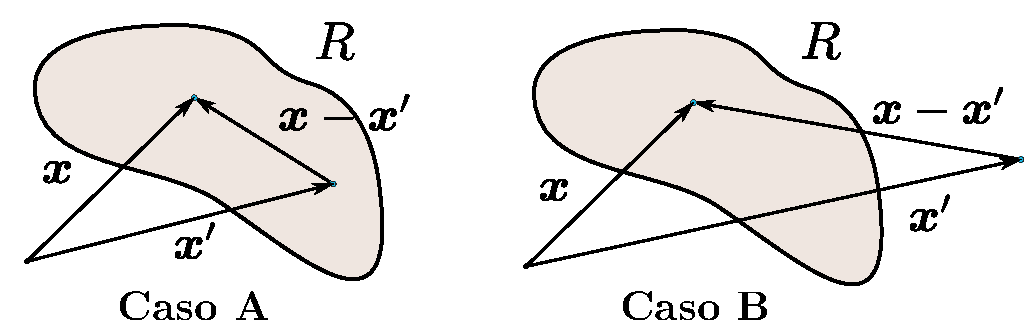
\includegraphics[width=0.8\textwidth]{images/fig_ft1_imagegreenCasos.pdf}	 
	\end{center}
	\caption{}
\end{figure} 
\[
	\psi = \frac{1}{|\vb{x}-\vb{x}'|} \qquad \lapm{\psi} = -4\pi \delta(\vb{x}-\vb{x}')
\]
\[
	-\phi(\vb{x})4\pi + \int_V 4\pi \frac{\rho(\vb{x}')}{|\vb{x}-\vb{x}'|} \; dV' =
	\int_S \left( \phi\dpar{\psi}{n}-\frac{1}{|\vb{x}-\vb{x}'|}\dpar{\phi}{n}\right)\; dS 
\]
donde estamos usando la abreviatura $\Nabla\phi\cdot\vb{n}=\partial\phi/\partial n$ que es la
derivada normal en la superficie. Despejando
\[
	\phi(\vb{x}) = \int_V \frac{\rho(\vb{x}')}{|\vb{x}-\vb{x}'|} \; dV' +
	\frac{1}{4\pi} \int_S \left( \frac{1}{|\vb{x}-\vb{x}'|}\dpar{\phi}{n} -\phi\frac{\partial}{\partial 
n} \left[\frac{1}{|\vb{x}-\vb{x}'|} \right] \right)\; dS ,
\]
donde la primer integral es debido a las cargas internas y la segunda al efecto de las cargas
fuera del reciento $R$.

Recordemos que las condiciones tipo Dirichlet corresponden a $\phi|_S$ y las tipo Neumann a
$\partial\phi/\partial \hat{n}|_S$.

El caso B, según figura, corresponde a
\[
	\rho_{int} \qquad \vb{x}'\notin R, \vb{x}\in R
\]
y 
\[
	\int_V \frac{\rho(\vb{x}')}{|\vb{x}-\vb{x}'|} \; dV' = 
	\frac{1}{4\pi} \int_S \left( \phi\frac{\partial}{\partial n} \left[\frac{1}{|\vb{x}-\vb{x}'|} \right]
	- \frac{1}{|\vb{x}-\vb{x}'|}\dpar{\phi}{n}  \right)\; dS ,
\]
la integral de superficie proviene de las cargas fuera de $R$ que producen campo en el interior
$R$.

Hemos tomado $\psi=1/|\vb{x}-\vb{x}'|$ que verifica [1]; interpretándose $\psi$ como el potencial
de una carga puntual unitaria.

\[
	\lapm{\frac{1}{|\vb{x}-\vb{x}'|}} = - 4\pi \delta( |\vb{x}-\vb{x}'| )
\]
podemos tomar
\[
	G \equiv \frac{1}{|\vb{x}-\vb{x}'|} + f( \vb{x}, \vb{x}')
\]
donde $G$ es la función de Green, el potencial de una carga unidad situada en $\vbx'$ calculado
en $\vbx$.
Luego, se tiene
\[
	\lapm{G} = -4\pi  \delta( \vb{x} - \vb{x}' ) + \lapm{f}
\]
donde $f$ satisface Laplace (si el reciento no incluye a $\vb{x}'$). 
Es decir que $\lapm{f( \vbx, \vbx' )} = 0$.

Entonces $f( \vb{x}, \vb{x}' )$ representan la o las imágenes necesarias para que
$G$ cumpla el contorno necesario $G_D|_S=0$.


% =================================================================================================
\section{Funciones de Green}
% =================================================================================================

El teorema de Green me da una expresión integral para el potencial $\phi$. En efecto,
\be
	\phi(\vb{x}) = \int_{V'} G(\vb{x},\vb{x}') \rho(\vb{x}')  \; dV' +
	\frac{1}{4\pi} \int_{S'} \left( G(\vb{x},\vb{x}')\dpar{\phi(\vbx')}{n} -\phi(\vbx')\frac{\partial}{\partial 
	n} G(\vb{x},\vb{x}') \right)\; dS' ,
	\label{green1}
\ee
y si $\vbx \notin V$, se tiene
\be
	0 = \int_{V'} G(\vb{x},\vb{x}') \rho(\vb{x}')  \; dV' +
	\frac{1}{4\pi} \int_{S'} \left( G(\vb{x},\vb{x}')\dpar{\phi}{n}(\vbx') -\phi(\vbx')\frac{\partial}{\partial 
	n} G(\vb{x},\vb{x}') \right)\; dS' .
	\label{green2}
\ee

Pero para poder utilizar \eqref{green1} necesito tener un solo tipo de condiciones de contorno,
de manera que según sean
\[
	\textrm{Dirichlet} \quad 	\begin{cases}
				G_D : \lapm{G_D} = -4\pi \delta(\vb{x},\vb{x}') \\
				G_D |_{contorno de R} = 0  \\
				\phi|_S \\
				\phi(\vb{x}) = \displaystyle \int_{V'} G_D \rho \; dV' - \frac{1}{4\pi}
				\int_{S} \phi|_S\frac{\partial}{\partial n} G_D \; dS'
			\end{cases}
\]
donde la condición de contorno de $G$ equivale, en el contexto físico del electromagnetismo, a
reemplazar el contorno por un conductor metálico puesto a tierra.
Entonces $G$ es el potencial de la configuración de conductores con el contorno puesto a tierra
frente a una carga puntual con magnitud unitaria.

La función de Green da la geometría del problema.

\[
	\dpar{\phi_1}{n}|_S - \dpar{\phi_2}{n}|_S = -4\pi\sigma \qquad \qquad \phi_2|_S = \phi_1|_S
\]

\[
	\textrm{Neumann} \quad 	\begin{cases}
				G_N : \lapm{G_N} = -4\pi \delta(\vb{x},\vb{x}') \\
				\Nabla G_N \cdot \hat{n}|_S = -\frac{4\pi}{S}  \\
				\left.\dpar{\phi}{n}\right|_S \\
				\phi(\vb{x}) = \displaystyle <\phi>|_S + \int_{V'} G_N \rho \; dV' + 
				\frac{1}{4\pi} \int_{S} G_N|_S \dpar{G_N}{n} \; dS
			\end{cases}
\]

\subsection{Función de Green libre}

La ecuación de Green libre
\[
	G(\vb{x}, \vb{x}') = \frac{1}{|\vb{x} - \vb{x}'|}
\]
que representa una superficie infinita con condición de contorno $\phi(|\vbx| \to \infty) = 0 $
lleva directo a la integral de Poisson. En efecto sería como no tener contornos (tenerlos en
infinito es no tenerlos).
Entonces 
\[
	\phi(\vb{x}) = \int_V G(\vbx,\vbx') \: \rho(\vbx') \:dV = 
	\int_{V'} \frac{ \rho(\vb{x}) }{|\vb{x}-\vb{x}'|} dV'
\]
que es la integral de Poisson. La ecuación de Poisson se recupera teniendo en cuenta
que
\[
	\nabla^2 \left( \frac{1}{|\vb{x} - \vb{x}'|} \right) = 4\pi \delta(\vb{x}-\vb{x}')
\]
% \[
% 	G(\vb{x}, \vb{x}') =  \frac{1}{|\vb{x} - \vb{x}'|} + f(\vb{x}, \vb{x}') \qquad 
% 	\textrm{con} \quad \lapm{f}(\vb{x}, \vb{x}') = 0 \quad \textrm{si} \quad \vb{x}\neq\vb{x}'
% \]
En este caso, Dirichlet y Neumann llevan a la misma solución porque potencial y campo son
nulos en los contornos.

\subsection{Sobre el caso de Neumann}

Para condiciones de Neumann se toma:
\[
	\Nabla G_N|_S = -\frac{4\pi}{S} = \left. \dpar{G}{n} \right|_S
\]
la integral 
\[
	- \frac{1}{4\pi} \int_S \phi|_S \left.\dpar{G}{n}\right|_S  dS
\]
no se puede anular con 
\[
	\left.\dpar{G}{n}\right|_S = 0
\]
salvo que el volumen de integración no contenga a $\vb{x}=\vb{x}'$ en cuyo caso:
se excluye $\vb{x}=\vb{x}'$ de la integración.
\[
	- \frac{1}{4\pi} \int_S \phi|_S \left.\dpar{G}{n}\right|_S  dS =
	\frac{1}{S} \int_S \phi|_S dS = <\phi>|_S
\]
que es el valor promedio de $\phi$ en la superficie $S$.

Se suele tomar la superficie $S \to \infty$ de modo que resulte nulo $<\phi>|_S$.
Se toma el volumen $V$ rodeado por dos superficies una cerrada y finita y la otra
en infinito entonces
\[
	<\phi>|_S = 0 \qquad \qquad \left. \dpar{G}{n}\right|_S = 0
\]
esto es el llamado {\it problema exterior}.

\subsection{Green para el problema externo de una esfera}

\notamargen{Este título sería ``Ejemplo método de imágenes''. En realidad este es un ejemplo
de cálculo de función de Green; así fue dado en la teoría.}

La configuración es una carga puntual $q$ frente a una esfera metálica de radio $a$ conectada a tierra.
La idea aquí es conocer dónde ubicar la imagen $ q' $ para que se verifique el contorno, es decir que
el potencial será ahora el correspondiente a las dos cargas 
\[
	\vp(\vbx) = \frac{q}{|\vbx - \vb{y}|} + \frac{q'}{|\vbx - \vb{y}'|} 
\]
y debe cumplir que 
\[
	\left. \vp(\vbx)\right|_{r=a} = 0,
\]
por la conexión a tierra. Para ajustar esta condición se tienen dos variables, la magnitud de la carga
$q'$ y su posición $\vb{y}'$.
No obstante, la simetría de la configuración establece ciertas restricciones para la posición $\vb{y}'$;
en efecto para el problema de una carga frente a una esfera el eje que une el centro de la esfera con
la carga es un eje de simetría de revolución; si la esfera gira en torno a ese eje la configuración es
la misma. Luego, la carga imagen debe ser tal que no rompa esa simetría: debe estar localizada en dicho
eje. Entonces $\vb{y}'$ y $\vb{y}$ son colineales y la posición incógnita requerida es solamente el
módulo $y'= |\vb{y}'|$.

Los módulos en los denominadores pueden expresarse en términos de la ley de los cosenos, como
\[
	\vp(\vbx) = \frac{q}{\sqrt{ x^2 + y^2 - 2 \: x \: y \:\cos{\gamma}} } +
	\frac{q'}{\sqrt{ x^2 + y'^2 - 2 \: x \: y' \cos{\gamma} }},
\]
donde $x, y$ son los módulos respectivos.

\begin{figure}[!htb]
	\begin{center}
	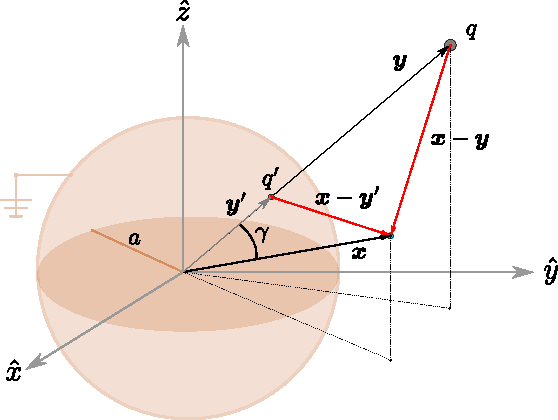
\includegraphics[width=0.5\textwidth]{images/fig_ft1_esfera_imagenes.pdf}
	\end{center}
	\caption{Geometría para el problema de la carga puntual $q$ frente a una esfera
	metálica de radio $a$ conectada a tierra.}
\end{figure} 

Luego, la condición de contorno evaluada sobre la superficie de la esfera $|\vb{x}| = a$ implica que 
\[
	\left. \vp(\vbx)\right|_{|\vb{x}| = a} = 
	\frac{q}{\sqrt{ a^2 + y^2 - 2 \: a \: y \:\cos{\gamma}} } +
	\frac{q'}{\sqrt{ a^2 + y'^2 - 2 \: a \: y' \: \cos{\gamma} }} = 0,
\]
y entonces se tienen que obtener ahora $q, y'$ a partir de esta ecuación que en realidad representan
infinitas direcciones dado que $ \gamma $ puede ser cualquier ángulo entre $0$ y $2\pi$.
Se necesitarán dos ecuaciones para resolver unívocamente el problema.
Si se eligen $\gamma = \pi$ y $\gamma = 0$ la ecuación anterior define el sistema
\notamargen{Parece ser una constante que si elegimos las cosas del modo más simétrico posible, las
expresiones resultan más sencillas.}
\[
	\begin{cases}
		\displaystyle \frac{q}{y-a} + \frac{q'}{a-y'} = 0 \\
		\\
		\displaystyle  \frac{q}{a+y} + \frac{q'}{a+y'} = 0 
	\end{cases}
\]
cuya solución es el par
\[
	q' = - \frac{a}{y} \: q, \qquad y' = \frac{a^2}{y},
\]
y entonces
\[
	\vp(\vbx) = \frac{q}{\sqrt{ x^2 + y^2 - 2 \: x \: y \:\cos{\gamma}} } -
	\frac{ ( a / y ) \: q }{ \sqrt{ x^2 + a^4 / y^2  - 2 \: x \:  ( a^2 / y ) \cos{\gamma} }}.
\]
El potencial en un punto $\vbx$ del espacio, debido a una carga en $\vb{y}$ depende de los módulos $x, y$ 
y del ángulo $\gamma$ entre dichos vectores.
\notamargen{Esta expresión, así como está, no se halla en ningún sistema de coordenadas en particular.}

Esta solución puede obtenerse un poco más heurísticamente, ver nota \ref{notas_carga_frente_a_esfera}.

Lo que sucede físicamente es que se induce carga sobre la superficie de la esfera.
Se querrá ver (luego?) cuál es la distribución de carga que se inducirá sobre la superficie.


\begin{figure}[htb]
	\begin{center}
	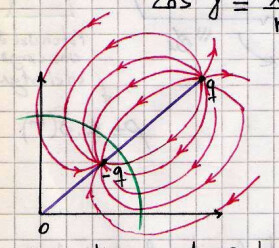
\includegraphics[width=0.4\textwidth]{images/fig_ft1_carga_induciendo_en_esfera.jpg}	 
	\end{center}
	\caption{}
\end{figure}

Este ejemplo ha servido también para mostrar la determinación de la funcion de Green para la configuración
dada por una esfera aterrizada (condiciones de Dirichlet), que sería
\[
	G(\vbx,\vb{y}) = \frac{1}{| \: \vbx - \vb{y} \:|} - \frac{a/|\vb{y}|}{| \:\vbx - ( a^2 / |\vb{y}| ) \hat{y} \: |} 
\]

% En este problema las condiciones adecuadas son las de Dirichlet, ver Figura,
% y podemos escribir la función de Green como 
% \[
% 	G = \frac{1}{|\vb{r} - D\hat{r}'|} - \frac{a/D}{|\vb{r} - a^2/D\hat{r}'|} \qquad G|_{r=a}
% \]
% sujeta a que 
% \[
% 	q' = -q a/D \qquad d = a^2/D
% \]
\begin{figure}[htb]
	\begin{center}
	\includegraphics[width=0.6\textwidth]{images/fig_ft1_green2.pdf}	 
	\end{center}
	\caption{$G_D$ es el potencial de la configuración (a) y se evalúa teniendo en cuenta la
	otra (b) que se resuelve casualmente por imágenes. La (c) se resuelve alterando las condiciones.}
\end{figure} 

El caso (c) de la Figura se resuelve con 
\[
	-\frac{V}{4\pi} \int_S \dpar{G}{n} dS = -\frac{V}{4\pi} \int_S \Nabla G\cdot d\vb{S} =
	-\frac{V}{4\pi} \int_V \lapm{G} \: dV	
\]
\[
	= -\frac{V}{4\pi} (-4\pi)\int_V \delta(\vb{x}-\vb{x}') \: dV	= V 
\]

\subsection{Algunos campos}

En distribuciones infinitas de carga la integral de Poisson diverge pero ello se debe a que en
realidad no existen distribuciones infinitas de carga.
% \begin{figure}[thb]
% 	\begin{center}
	\includegraphics[width=0.8\textwidth]{images/fig_ft1_campohilos.pdf}	 
% 	\end{center}
% 	\caption{}
% \end{figure} 

\begin{ejemplo}{\bf Problema 1}

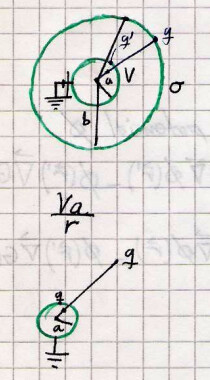
\includegraphics[width=0.2\textwidth]{images/fig_ft1_g1_p1_A.jpg} 

Primeramente se calculan los valores de la carga imagen, los cuales, para un
sistema de coordenadas esféricas, son
\[
	q'= -\frac{a}{r} q \qquad r'= \frac{a^2}{r}.
\]
Se ve que cumplen los límites razonables.
Luego, habría que hacer el potencial nulo mandando el engendro a tierra y luego se
le suma algo que de potencial $V$ en $r=a$.

La función de Green por imágenes será
\[
	G_D = \frac{1}{|\vbx - \vbx'|} - \frac{1}{r'|\vbx - a^2/r'^2 \vbx'|},
\]
la cual cumple que sobre la superficie es nula.

Subsecuentemente,
\[
	\rho(\vbx') = \sigma \delta(r-b), \phi(\vbx')|_S = V, \phi(\vbx')|_{S_{R\to\infty}} = 0 
\]
y
\[
	\int \rho(\vbx') \: dV = 4 \pi b^2 \sigma 
\]
\[
	\int \rho(\vbx') \: G_D( \vbx, \vbx')  \: dV = \int \frac{b^2 \sigma}{|\vbx - \vbx'|} \: dS
\]
siendo $b=|\vbx'|$. Poniendo manos a la obra en la integral (en esféricas)
\[
	\int \frac{b^2 \sigma}{|\vbx - \vbx'|} \: dS =
	\int dt \int d\Omega r^2 \sigma \delta(r'-b) 
	\left[ \frac{1}{|\vbx - \vbx'|} - \frac{1}{r'|\vbx - a^2/r'^2 \vbx'|} \right]
\]
\[
	\int d\Omega \sigma b^2
	\left[ \frac{1}{|\vbx - \vbx'|} - \frac{1}{r'|\vbx - a^2/r'^2 \vbx'|} \right]
\]
donde el primer término es el potencial de un casquete, que es 
\[
	\begin{cases}
	 \displaystyle \frac{4\pi b^2\sigma}{r} \quad \text{ si } \; r > b \\
	 \\
	 \displaystyle 4 \pi b^2 \sigma \quad \text{ si } \; a < r < b 
	\end{cases}
\]
y el segundo término se puede trabajar para llegar a
\[
	\frac{b^2 a }{r} \int d\Omega \sigma \frac{-1}{|a^2/r^2 \vbx - \vbx'|} 
\]
Pero recordemos que 
\[
	\dpar[2]{\vbx}{r} = \frac{a^2}{r} < a
\]

Juntando todo
\[
	\begin{cases}
	 \displaystyle \frac{4\pi b^2\sigma}{r} - \frac{a}{r} 4 \pi \sigma b \qquad \text{ si } \; r > b \\
	 \\
	 \displaystyle  4 \pi b^2 \sigma - \frac{a}{r} 4 \pi \sigma b \qquad \text{ si } \; a < r < b  
	\end{cases}	
\]

Y se tiene 
\[
	-\frac{ 1 }{ 4\pi } \int \phi(\vbx') \Nabla' G_D(\vbx,\vbx') dS' =
	\frac{ V }{ 4 \pi } \int \Nabla' G_D(\vbx,\vbx') dS' = V Q_n,
\]
donde en el último paso se ha usado el teorema de la divergencia. Luego, como
$Q_n = -a/r$ se tiene 
\[
	\phi = \frac{Va}{r}
\]
que entonces en $r=a$ es $V$.

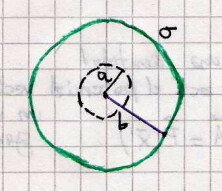
\includegraphics[width=0.2\textwidth]{images/fig_ft1_g1_p1_B.jpg} 

Esto conviene hacerlo integrando en esféricas con $\vbx \parallel \hat{z}$.

\end{ejemplo}

\begin{ejemplo}{\bf Comentario superposición}
 
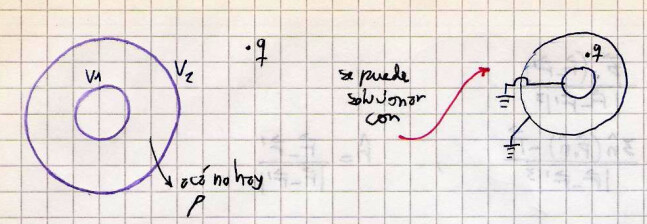
\includegraphics[width=0.5\textwidth]{images/fig_ft1_comentario_superposicion.jpg} 
 
\end{ejemplo}

% =================================================================================================
\section{Condiciones de contorno para el campo eléctrico}
% =================================================================================================

Consideraremos la superficie de separación entre dos medios 1 y 2, la cual puede estar cargada, y sobre
la misma imaginaremos un cilindro pequeño $\Sigma$ de tapas paralelas a la superficie y altura despreciable y 
asimismo, un circuito cerrado $\Gamma$ también de altura despreciable perpendicular a la superficie, ver figura.

La normal a la superficie es $\hat{n}$ mientras que $\hat{t}$ es un versor tangente a la misma.

\begin{figure}[!htb]
	\begin{center}
	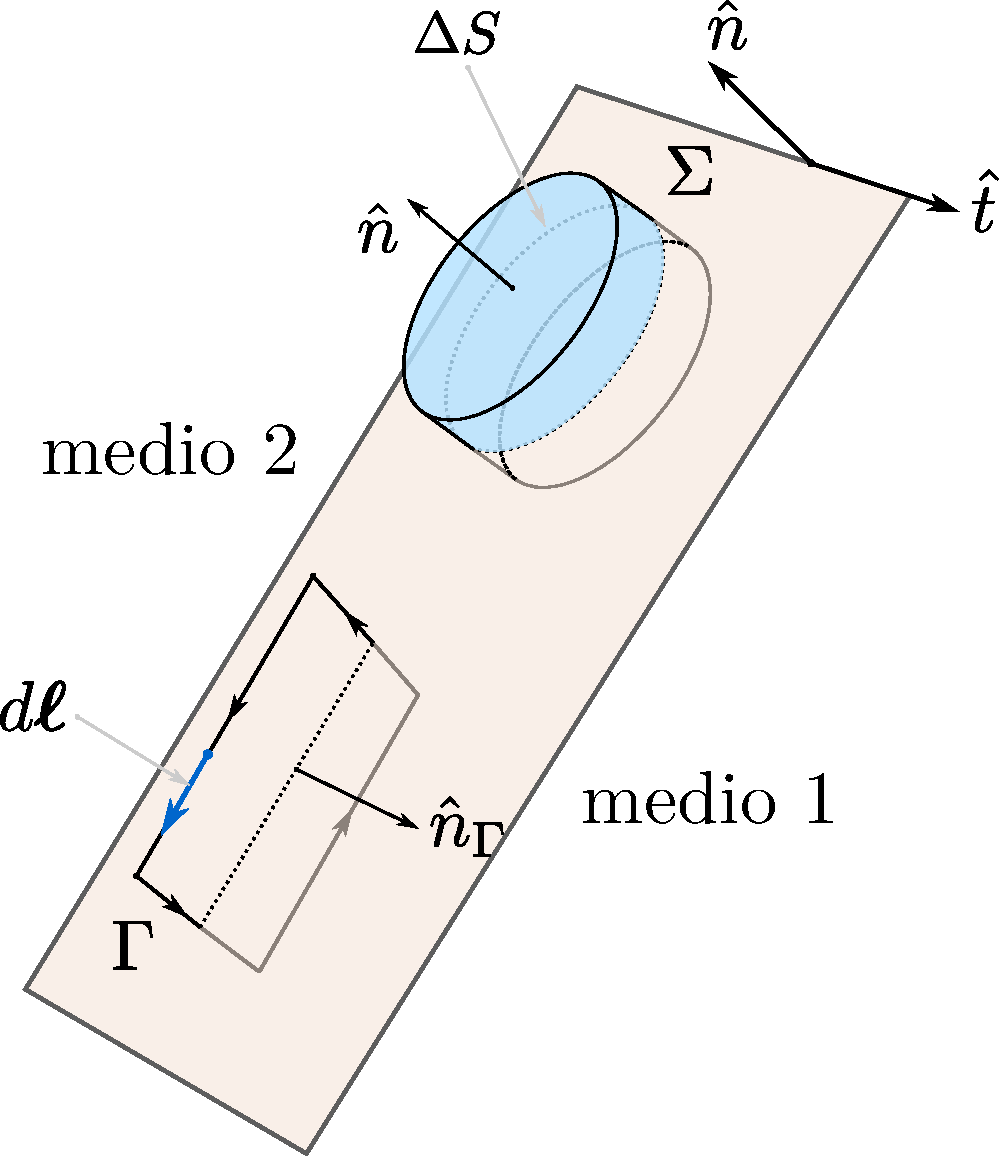
\includegraphics[width=0.4\textwidth]{images/fig_ft1_contornos_E.pdf} 
	\end{center}
	\caption{}
\end{figure} 

La ley de Gauss establece para el cilindro $\Sigma$ que 
\[
	\int_{S_\Sigma} \vb{E} \cdot d\vb{S} = 4 \pi \: Q_n,
\]
donde $ {S_\Sigma}$ es la superficie total del cilindro y $Q_n$ la carga neta encerrada.
Como la superficie lateral es despreciable, por serlo la altura, la integral de superficie se reduce a la
de las tapas. Si la densidad de carga sobre la superficie es $\sigma$ entonces
\[
	( \vb{E}_2 - \vb{E}_1 )\cdot \hat{n} \: \Delta S = 4 \pi \: \sigma \: \Delta S 
\]
o bien
\[
	( \vb{E}_2 - \vb{E}_1 )\cdot \hat{n} = 4 \pi \sigma 
\]
lo cual implica que la componente normal del campo $\vb{E}$ es discontinua si hay carga superficial presente.

\notamargen{No sé si no decir directamente que en electrostática es nula la integral de línea de E y ya.}
Por otra parte, como el rotor de $\vb{E}$ es nulo (en electrostática), el teorema de Stokes implica
\[
	\int_{S} \: \rotorm{E} = 0 = \int_{\Gamma} \vb{E} \cdot d\Bell
\]
y despreciando el aporte de las partes del circuito que son perpendiculares a la superficie, resulta
\[
	( \vb{E}_2 - \vb{E}_1 ) \cdot d\Bell  = 
	( \vb{E}_2 - \vb{E}_1 ) \cdot ( \hat{n}_\Gamma \times \hat{n} ) \: d\ell = 0
\]
donde en el miembro derecho se ha expresado la dirección del $d\Bell$ en función de los versores
normal y tangencial, y entonces
\[
	\hat{n}_\Gamma \cdot ( \hat{n} \times  ( \vb{E}_2 - \vb{E}_1 ) ) = 0,
\]
que indica que el segundo factor tiene que ser nulo, es decir 
\[
	 \hat{n} \times  ( \vb{E}_2 - \vb{E}_1 ) = 0
\]
y esto implica que la componente tangencial del campo es continua, sin importar que exista carga o no.
\notamargen{Acordate que harcodeaste con un pdf el $\ell$ bold.}

Entonces el trabajo yendo del medio 1 al 2 será nulo
\[
	W_{1\to 2} = 0 = q ( \phi_2 - \phi_1 ),
\]
lo cual implica que $\phi_2 = \phi_1$ porque la discontinuidad del campo es finita.
Como veremos luego, esto no vale en el caso de una capa dipolar.
\notamargen{Hay que ver la relación de esto con lo anterior; creo que no estoy entendiendo, o explicando,
bien.}

Resumiendo
\[
	E_{2\hat{n}} - E_{1\hat{n}} = 4 \pi \sigma \qquad \qquad E_{2\hat{t}} -E_{1\hat{t}} = 0
\]

Expresando el campo en términos del potencial, se tiene
\[
	-\Nabla\phi_2\cdot\hat{n} + \Nabla\phi_1\cdot\hat{n} = 4 \pi \sigma
\]
\[
	\frac{\Nabla(\phi_2-\phi_1)\cdot \hat{n}}{4 \pi} = \sigma
\]
\be
	\sigma = \frac{1}{4\pi}\dpar{(\phi_1-\phi_2)}{n}
	\label{densidad_de_carga}
\ee
esta es la densidad de carga inducida sobre la frontera entre medios.

\subsection{Carga puntual frente a esfera puesta a tierra}

Volvemos a este problema, recordando que el potencial fuera de la misma se hubo determinado por el método
de imágenes. Recordemos también que dentro de la esfera el potencial debe ser constante (no hay carga allí,
puesto que la imagen es un dispositivo virtual sin existencia física).
Consideramos dos secciones, interna y externa.

Por la simetría del problema la densidad de carga inducida tiene la simetría de revolución en torno al 
eje que pasa por $q, q'$ y el origen de coordenadas y será máxima en el punto de la esfera más cercano a
$q$.
Dado que el potencial es constante dentro de la esfera, e igual al valor que toma sobre la superficie, la
ecuación \eqref{densidad_de_carga} es 
\[
	\sigma = - \frac{1}{4\pi} \left.\dpar{\vp}{n}\right|_S.
\]
Ubicando nuestra esfera en el origen de un sistema de coordenadas esféricas, la normal externa $\hat{n}$
es claramente $\rver$ de modo que derivar normalmente es derivar con respecto a la dirección radial, es 
decir $\partial / \partial n \equiv \partial / \partial r$ y entonces 
\[
	\sigma = - \frac{1}{4\pi} \left.\dpar{\vp}{r}\right|_{r=a} =
	- \frac{q}{4 \pi a^2} \Frac{a}{y} 
	\frac{[ 1 - (a / y)^2 ]}{[\: 1 + (a / y)^2 - 2 \: (a/y) \: \cos \gamma \:]^{3/2}}.
\]
\notamargen{La definición de derivada normal puede ir para apéndice.}

Si consideramos ahora el problema interno; esto es, una carga q rodeada por una esfera conductora conectada
a tierra, se pueden hacer los mismos razonamientos que en el caso de la carga exterior y la solución es la
misma intercambiando $q'$ por $q$ y $y'$ por $y$.
Entonces, en ese caso el cálculo de la densidad utiliza $\hat{n} = -\rver$ y se tiene 
\[
	\sigma = \frac{1}{4\pi} \left.\dpar{\vp}{r}\right|_{r=a} =
	- \frac{q}{4 \pi a^2} \Frac{a}{y} 
	\frac{[ (a / y)^2 - 1 ]}{[\: 1 + (a / y)^2 - 2 \: (a/y) \: \cos \gamma \:]^{3/2}}
\]
\notamargen{Acá debiera estar claro que se invierte el significado de $y'$, ahora es mayor que $a$.}

La carga total inducida sobre una superficie se evaluará en general a través de
\[
	Q = \int_S \: \sigma \: dS.
\]

En el caso anterior del problema de la carga frente a una esfera a tierra se puede utilizar la ley de Gauss
para hallar en cada caso la carga total de una manera inmediata.

% \begin{figure}[hb]
% 	\begin{center}
	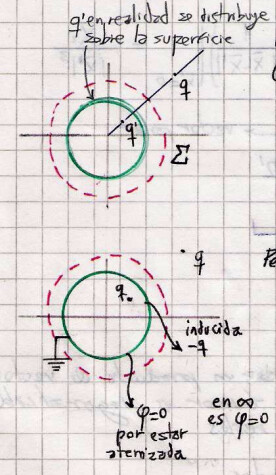
\includegraphics[width=0.25\textwidth]{images/fig_ft1_calculo_carga_fast.jpg}	 
% 	\end{center}
% 	\caption{}
% \end{figure} 

Situando una superficie gaussiana $\Sigma$ por fuera de la esfera, como se ve en la figura, resulta que la
carga encerrada neta es la misma con imagen o sin imagen. En efecto, en el problema real la carga encerrada
se distribuye sobre la superficie mientras que en el problema equivalente está concentrada en la posición
$y'$ y sabemos que es $q'$; luego como los dos problemas son equivalentes el lado derecho de la ley de 
Gauss debe ser idéntico y la carga inducida será la neta encerrada, que es $q'$, la carga imagen.

Procediendo de modo similar para el problema interno (ahora $q'$ está por fuera de la superficie $\Sigma$),
ahora la situación es diferente porque el campo sobre \Sigma es nulo (solo es no nulo fuera de la esfera
por la conexión a tierra). Entonces la ley de Gauss ya nos dice ahí que la carga neta es nula y ello
lleva a que la carga inducida sea $-q$ que no es igual a la carga imagen.


\subsection{Principio de superposición}

Consideremos la situación depicted en la figura

\begin{figure}[htb]
	\begin{center}
	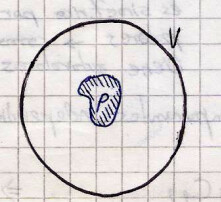
\includegraphics[width=0.2\textwidth]{images/fig_ft1_rho_rodeada_por_V.jpg}	 
	\end{center}
	\caption{}
\end{figure} 

Una cierta distribución de carga está rodeada por una superficie a potencial $V$.
El potencial en un punto $\vbx$ es
\[
	\vp(\vbx) = \int_\Omega \rho(\vbx') \: G_D(\vbx,\vbx') \: d\Omega 
	- \frac{1}{4\pi} \int \vp \dpar{G}{n} \: dS
\]
pero como el potencial sobre la superficie está fijo en $V$ la última integral es 
\[
	- \frac{1}{4\pi} \int \vp \dpar{G}{n} \: dS = - \frac{V}{4\pi} \int \Nabla G \cdot\hat{n} \: dS,
\]
la cual por el teorema de la divergencia resulta
\[
	- \frac{V}{4\pi} \int \Nabla G_D \cdot\hat{n} \: dS =
	- \frac{V}{4\pi} \int_V \Nabla \cdot (\Nabla G_D) \: dV =
	- \frac{V}{4\pi} \int_V \lapm{G_D} \: dV
\]
y recordando que la función de Green es solución de la ecuación de Poisson para una densidad dada por
la delta de Dirac, se tiene
\[
	- \frac{V}{4\pi} \int \Nabla G_D \cdot\hat{n} \: dS = 
	V \int \delta(\vbx - \vbx') \: dV = V,
\]
de manera que 
\[
	\vp{\vbx} = \int_\Omega \rho(\vbx') \: G_D(\vbx,\vbx') \: d\Omega  + V,
\]
lo cual puede una manera de ver el principio de superposición.


\textbf{Notas importantes sobre el principio de superposición}

La ecuación de Poisson es muchas veces inútil porque en general no se tiene la distribución de cargas
$ \rho(\vbx) $. Esto sucede en general con conductores pués la carga allí se distribuye acomodándose
para alcanzar el equilibrio.

Para campos y potenciales vale superposición.
Pero cada problema de potencial (con su ecuación de poisson) incluye además de la ecuación las condiciones
de contorno. 
Dados dos problemas
\[
	\nabla^2 \vp_1 = - 4 \pi \rho_1 \qquad + \qquad \text{CC}_1
\]
y
\[
	\nabla^2 \vp_2 = - 4 \pi \rho_2 \qquad + \qquad \text{CC}_2
\]
la suma de soluciones $ \vp = \vp_1 + \vp_2 $ con $\rho = \rho_1 + \rho_2 $
\be
	\nabla^2 \rho = - 4 \pi \rho \qquad + \qquad \text{CC}
	\label{problema_potencial_suma}
\ee
donde hay que asegurarse de que $ \text{CC} $ sea la suma de las condiciones del problema 1 y las del
problema 2.
Desde el otro punto de vista, si tengo un problema como \eqref{problema_potencial_suma} y lo quiero
pensar como la superposición de dos potenciales $ \vp = \vp_1 + \vp_2 $ puedo generarme unas condiciones
de contorno artificiales que tengan en cuenta las influencias mutuas.

\notamargen{Habría que entender bien este tema que es crucial. Imagino que working los ejemplos podría
recuperar lo que alguna vez supe.}

\subsection{Condiciones de contorno para medios magnéticos}

Para los medios magnéticos
\[
	\rotorm{H} = \frac{4 \pi}{c} \vb{J}_l
\]
\[
	\int_S (\rotorm{H}) \cdot d\vb{S} = \int_S \frac{4 \pi}{c} \vb{J}_l \cdot d\vb{S} = 
	\frac{4 \pi}{C} \vb{g}_l\cdot \hat{s} d\ell
\]
donde hicimos la transformación
\[
	\int \vb{H}\cdot d\ell = (\vb{H}_2-\vb{H}_1)\cdot d\ell
\]
y donde recordemos que la altura de $\Gamma$ tiene a cero.
\[
	\frac{4 \pi}{c} \vb{g}_l \cdot \vb{s} = ( -\vb{H}_2 + \vb{H}_1 )\cdot( \hat{n} \times \hat{s} ) d\ell
\]
\[
	\frac{4 \pi}{c} \vb{g}_l \cdot \vb{s} \; d\ell = (\vb{H}_1 -\vb{H}_2 \times \hat{n})\cdot \hat{s} 
d\ell
\]

\begin{figure}[htb]
	\begin{center}
	\includegraphics[width=0.4\textwidth]{images/fig_ft1_contorno2.pdf}	 
	\end{center}
	\caption{}
\end{figure} 

de manera que 
\[
	\frac{4 \pi}{c} \vb{g}_l = \hat{n} \times ( \vb{H}_2 - \vb{H}_1 )
\]
\[
	\hat{n}\times\hat{s} = \frac{d\vb{\ell}}{d\ell} 
\]
\[
	B_{2\hat{n}} - B_{1\hat{n}} = 0 \qquad \qquad H_{2\hat{t}} - H_{1\hat{t}} = \frac{4 \pi}{c} g_l
\]
\[
	\int_S \vb{B}\cdot d\vb{S} = 0 \Rightarrow (\vb{B}_2 - \vb{B}_1 )\cdot\hat{n} = 0
\]

% =================================================================================================
\section{Desarrollo multipolar}
% =================================================================================================

Si se conoce la distribución de carga el potencial se obtiene integrando
\be
	\phi(\vb{x}) = \int_{V'} \frac{ \rho( \vbx' ) }{| \vbx -\vbx' | } \; dV'.
	\label{integral_potencial}
\ee

No obstante, esta expresión puede ser muy complicada porque en el denominador depende de la variable 
$\vbx'$ sobre la cual se está integrando. 
Resulta conveniente entonces hacer un desarrollo del denominador, que es una función de $\vbx'$, en
torno a un punto que se toma como origen de una esfera que engloba a la distribución de carga.
Luego, ese dearrollo será válido en puntos externos a dicha esfera.

\notamargen{Se necesita una serie que converja, y que lo haga rápido.
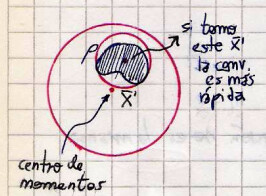
\includegraphics[width=0.3\textwidth]{images/fig_ft1_expansion_multipolar.jpg}}

Entonces, desarrollando en torno a $\vbx'=0$ (el origen de coordenadas) se tienen
\[
	\frac{ 1 }{| \vbx -\vbx' | } = 
	\frac{ 1 }{| \vbx |} + \left.\partial_i \left( \frac{ 1 }{| \vbx -\vbx' | } \right)\right|_{\vbx'=0} x_i' +
	\frac{1}{2} \: \left. \partial_j \partial_i \left( \frac{ 1 }{| \vbx -\vbx' | } \right)\right|_{\vbx'=0} x_i' x_j' + ...,
\]
o bien 
\[
	\frac{ 1 }{| \vbx -\vbx' | } = 
	\frac{ 1 }{| \vbx |} + \frac{x_i \: x_i'}{| \vbx |^3} +
	\frac{1}{2} \frac{ x_i \: x_i' \: x_j \: x_j' }{ | \vbx |^5 } + ...,	
\]
\notamargen{Chequear la expansión, tal vez ponerla en vectorial o hacerla bien en el Apéndice.
Juntar huevos y hacer el término siguiente.}
Luego, introduciendo la misma en \eqref{integral_potencial} resulta
\begin{multline*}
 	\phi(\vb{x}) =
	\frac{ 1 }{| \vbx |} \int_{V'} \rho( \vbx' ) \: dV' + 
	\frac{x_i }{| \vbx |^3} \: \int_{V'} \: x_i' \: \rho( \vbx' ) \: dV' + \\
	\frac{1}{2} \frac{ x_i  \: x_j  }{ | \vbx |^5 } 
	\int_{V'} \: (\: 3 x_i' \: x_j' - \delta_{ij}|\vbx|^2 \:) \: \rho( \vbx' ) \: dV' + ...,
\end{multline*}
% \[
% 	\phi(\vb{x}) =
% 	\frac{ 1 }{| \vbx |} \int_{V'} \rho( \vbx' ) \: dV' + 
% 	\frac{x_i }{| \vbx |^3} \: \int_{V'} \: x_i' \: \rho( \vbx' ) \: dV' +
% 	\frac{1}{2} \frac{ x_i  \: x_j  }{ | \vbx |^5 } 
% 	\int_{V'} \: (\: 3 x_i' \: x_j' - \delta_{ij}|\vbx|^2 \:) \: \rho( \vbx' ) \: dV' + ...,
% \]

Se tiene un desarrollo de diferentes órdenes 
\[
	\phi(\vb{x}) = \phi^{(0)}(\vbx) + \phi^{(1)}(\vbx) + \phi^{(2)}(\vbx) + \phi^{(3)}(\vbx) + ...
\]
que se conocen según
\[
	\frac{ 1 }{| \vbx |} \int_{V'} \rho( \vbx' ) \: dV' = \frac{ Q }{| \vbx |} \qquad \text{ Orden monopolar }
\]
\[
	\frac{x_i }{| \vbx |^3} \: \int_{V'} \: x_i' \: \rho( \vbx' ) \: dV' = 
	\frac{x_i \: p_i }{| \vbx |^3} \: \qquad \text{ Orden dipolar }
\]
\[
	\frac{1}{2} \frac{ x_i  \: x_j  }{ | \vbx |^5 } 
	\int_{V'} \: (\: 3 x_i' \: x_j' - \delta_{ij}|\vbx|^2 \:) \: \rho( \vbx' ) \: dV' =
	\frac{1}{2} \frac{ x_i  \: Q_{ij} \: x_j  }{ | \vbx |^5 } \qquad \text{ Orden cuadrupolar }
\]
% \[
% 	\qquad \text{ Orden octupolar }
% \]

El último término, matricialmente sería
\[
	\frac{1}{2} \frac{\vb{x}^t Q \vb{x}}{|\vb{x}|^5}.
\]

Los momentos son el momento monopolar,
\[
	Q = \int_V \rho(\vb{x}) dV, 
\]
que es la carga total, el momento dipolar,
\[
	\vb{p} = \int_V \vb{x} \: \rho(\vb{x}) \: dV
\]
y el momento cuadrupolar
\[
	Q_{ij} = \int_V  \rho(\vb{x}) \left[ 3 x_i x_j - \delta_{ij} |\vb{x}|^2 \right] \: dV
	= 3 \int_V  \rho(\vb{x}) x_i \: x_j  \: dV - \delta_{ij} \int_V  \rho(\vb{x})  |\vb{x}|^2  \: dV
\]
\[
	Q_{ij} = 3 C_{ij} - \delta_{ij} C_{ll},
\]
donde esta última expresión permite ver que el momento cuadrupolar es de traza nula ($C_{ll}$ es la traza).

El momento cuadrupolar refleja apartamiento de la esfera perfecta, los momentos dipolar y cuadrupolar
indican desbalance de carga.
Asimismo $Q_{ij} = Q_{ji}$ es simétrico por ser producto de vectores polares.
Es siempre diagonalizable y tiene autovalores reales. 
Tiene traza nula,
\[
	Q_{xx} + Q_{yy} + Q_{zz}  = 0
\]

El tensor diagonalizado tendrá tres componentes independientes.


Se da también que $Q_{ij} (i\neq j)$ mide desbalance lejos de los ejes.
Una esfera con $\rho$ uniforme tiene todos los momentos multipolares nulos salvo el monopolo.

\begin{figure}[htb]
	\begin{center}
	\includegraphics[width=0.8\textwidth]{images/fig_ft1_multipolo2.pdf}	 
	\end{center}
	\caption{}
\end{figure}

\notamargen{El comentario en pag. 12 de la carpeta -recuadrado en rojo- induce algo diferente;
pide simetría en el plano perpendicular al vector. Me parece a mí que lo que debiera verse es
una simetría en la distribución de carga.}
Una simetría de reflexión implica que el $\vb{p}_\perp = 0$ donde la notación significa perpendicular
al plano. Esto es así porque no hay desbalance. Para una simetría de revolución $Q_{xx}=Q_{yy}$ entonces
el $Q_{ij}$ puede darse con un sólo número.

Si en una distribución dada, los momentos multipolares hasta el orden $\ell -1$ son nulos entonces
el momento multipolar de orden $\ell$ no depende del origen de coordenadas.
Así, por ejemplo, cuando el monopolo es nulo el momento dipolar no depende del centro de momentos.

\begin{figure}[htb]
	\begin{center}
	\includegraphics[width=0.6\textwidth]{images/fig_ft1_multipolo3.pdf}	 
	\end{center}
	\caption{}
\end{figure}

En la figura vemos que no ambos no tienen desbalance de carga respecto del origen; el disco uniformemente
cargado tendrá monopolo no nulo y dipolo nulo (siempre respecto del origen), los anillos cargados con carga
opuesta tendrán monopolo y dipolo nulos (respecto del origen y de cualquier otro punto). Pero si muevo las
distribuciones se tendrá desbalance el disco pero no los anillos.

\begin{figure}[htb]
	\begin{center}
	\includegraphics[width=0.3\textwidth]{images/fig_ft1_multipolo4.pdf}	 
	\end{center}
	\caption{}
\end{figure}

Para átomos en general son monopolo, dipolo neutros; el cuadrupolo se da con un solo número. 
En la Figura tenemos un elipsoide con densidad de carga $\rho$ uniforme. Tiene simetría de revolución
de modo que el momento cuadripolar es un número. $Q_{zz} = 0 $ puesto que una esfera no tiene
desbalance, entonces $\overleftrightarrow{Q} = 0 $ 

Para una esfera uniformemente cargada todos los momentos dipolares más allá del monopolo valen
cero, lo cual se ve por ley de Gauss.

En general en las aplicaciones uno se queda con tres términos; monopolo, dipolo y cuadrupolo y se
busca que esa expresión converja rápido. En general tomando como centro el centro de la distribución
la convergencia es más rápida.


% =================================================================================================
\section{Dipolo eléctrico}
% =================================================================================================

Se obtiene como límite de 
\[
	\phi(\vb{x}) = \frac{ q }{| \vbx - \vbx_+ |}  - \frac{ q }{| \vbx - \vbx_- |}.
\]
\notamargen{No sé si corresponde hacer mención a que el potencial del dipolo se obtiene como 
límite en el caso de que la distancia entre cargas tiende a la nulidad.}

El potencial de un dipolo es
\[
	\phi(\vb{x}) = \frac{ \vb{p}\cdot\vb{x} }{|\vb{x}|^3} 
\]
si está en el origen, y
\[
	\phi(\vb{x}) = \frac{ \vb{p}\cdot(\vb{x}-\vb{x}_0) }{|\vb{x} - \vb{x}_0|^3} 
\]
si está en un punto $\vb{x}_0$. Para calcular el campo hay que tomar el gradiente de esta expresión,
multiplicarlo por $-1$, lo cual es un poco trabajoso, pero ahí vamos.
Usando que el segundo miembro es a su vez un gradiente [poner esa cuenta en el apéndice matemático]
se tiene 
\[
	\vb{E}(\vb{x}) = -\Nabla \phi(\vbx) = 
	-\Nabla \left( \frac{ \vb{p}\cdot(\vb{x}-\vb{x}_0) }{|\vb{x} - \vb{x}_0|^3} \right) =
	\Nabla \left( \vb{p} \cdot \Nabla\left( \frac{ 1 }{|\vb{x} - \vb{x}_0|} \right) \right),
\]
luego se utiliza la identidad para el gradiente de un producto escalar notando que como uno de
los vectores en el escalar es a su vez un gradiente se tiene una expresión más sencilla 
[otra cuenta de apéndice]
\notamargen{La identidad es $\Nabla(\pe{A}{B}) =$ cuatro términos, dos rotores y dos
términos del tipo convectivo.}
En efecto, el primer término se anula por involucrar el producto vectorial de un gradiente, el
segundo y tercero porque $\vb{p}$ es independiente de $\vbx$ reduciéndose la expresión a
\[
	\vb{E}(\vb{x}) = (\vb{p}\cdot\Nabla) \Nabla\left( \frac{ 1 }{|\vb{x} - \vb{x}_0|} \right)
\]
que implica que el operador $\Nabla$ que multiplica al momento dipolar se aplica sobre el gradiente
de $1/|\vb{x} - \vb{x}_0|$. Ahora restauramos ese último valor y la cuenta se 
puede hacer más fácilmente en indicial [la hago como nota al final]. 
Finalmente
\[
	\vb{E}(\vb{x}) = \frac{3 \vb{p}\cdot\hat{n} }{|\vb{x} - \vb{x}_0|}  \hat{n} - 
		\frac{ \vb{p} }{|\vb{x} - \vb{x}_0|^3}	
\]
donde 
\[
	\hat{n} = \frac{\vb{x}-\vb{x}_0}{|\vb{x}-\vb{x}_0|}.
\]

\begin{figure}[htb]
	\begin{center}
	\includegraphics[width=0.3\textwidth]{images/fig_ft1_dipolar2.pdf}	 
	\end{center}
	\caption{Dipolo centrado en el origen.}
\end{figure}

Si hacemos una transformación ortogonal de cartesianas a esféricas para un dipolo con \vb{p} en 
el eje $z$, se tiene 
\[
	\begin{pmatrix}
	 p_r \\ p_\theta \\ p_\vp
	\end{pmatrix} =
	\begin{pmatrix}
	 \sin \theta \cos \vp & \sin \theta \sin \vp & \cos \theta \\
	 \cos \theta \cos \vp & \cos \theta \sin \vp & -\sin \theta \\
	 -\sin \vp & \cos \vp & 0
	\end{pmatrix}
	\begin{pmatrix}
	 0 \\ 0 \\ p
	\end{pmatrix}
\]
\notamargen{Pasarla al apéndice esta matriz.}
y para este caso particular son el potencial
\[
	\phi(\vb{x}) = \frac{p\hat{z}\cdot r\hat{r}}{r^3} = \frac{p}{r^2} \cos(\theta)
\]
y el campo
\[
	\vb{E}(r,\theta) = \frac{2 p\cos(\theta)}{r^3} \hat{r} + \frac{p\sin(\theta)}{r^3} \hat{\theta}
\]
que tiene simetría de revolución, puesto que no depende de $\phiver$.

Las líneas de campo cumplen que un diferencial de arco $d\Bell$ a través de una línea de campo es tal que 
\[
	d \Bell \parallel \vb{E} \quad \Rightarrow \quad  \vb{E} \times d\Bell = 0
\]
la línea de campo sigue la dirección del campo. 

En coordenadas curvilíneas generales es
\[
	d\Bell = h_1 dq_1 \hat{e}_1 + h_2 dq_2 \hat{e}_2 + h_3 dq_3 \hat{e}_3
\]
y para un campo cualquiera $\vb{E} = E_1 \hat{e}_1 + E_2 \hat{e}_2 + E_3 \hat{e}_3$ se verificarán
\[
	\frac{h_1 dq_1}{E_1} = \frac{h_2 dq_2}{E_2} = \frac{h_3 dq_3}{E_3}
\]
En el caso de esféricas $ h_1 = 1, h_2 = r, h_3 = r \sin \theta $ y evaluando el producto vectorial
resulta $ dr/r = 2 \cotg \theta \: d\theta $, las líneas de campo, en el caso del dipolo no tendrán componente
en $\phiver$ (como es de esperar).

\subsection{Independencia del origen para el momento dipolar}

Queremos ver el hecho de que si los momentos de orden $\ell-1$ son nulos entonces el momento de orden $\ell$
no depende del origen.
Escribimos el momento dipolar de orden $\ell$ como
\[
	Q^{\ell}_{\alpha\beta\gamma} \propto \int \rho(\vbx) \: x^\alpha y^\beta z^\gamma  \: d^3x
\]
donde $\ell = \alpha + \beta + \gamma$.
Trasladamos el origen del sistema de coordenadas $\vbx'= \vbx - \vbx_0$, entonces
\[
	Q^{\ell}_{\alpha\beta\gamma} \propto \int \rho(\vbx') \: (x'+x_0)^\alpha (y'+y_0)^\beta (z'+z_0)^\gamma  \: d^3x',
\]
y usamos combinatoria allí
\[
	( x + c )^n = \sum_{r=0}^n \left( \frac{n}{r} \right) x^{n-r} c^r,
\]
\notamargen{Poner el símbolo correcto del combinatorio}
donde $(n r) = n! / ( (n-r)! r! )$ de manera que 
\[
	Q^{\ell}_{\alpha\beta\gamma} \propto \sum_{rst}^{\alpha\beta\gamma} 
	\left( \frac{\alpha}{r} \right) \left( \frac{\beta}{s} \right) \left( \frac{\gamma}{t} \right)
	x_0^r \: y_0^s \: z_0^t \:
	\int \rho(\vbx') \: {x'}^\alpha {y'}^\beta {z'}^\gamma  \: d^3x'
\]
donde $0\leq r\leq \alpha, 0\leq s\leq \beta$ y $0\leq t\leq \gamma$.
Si $r=s=t=0$ entonces tenemos el multipolo de orden \ell calculado en el sistema $X'Y'Z'$.

Esto es general; si en una distribución monopolo y dipolo son nulos entonces el cuadripolo no depende
del origen de coordenadas.  
\notamargen{Esto ya se dijo mucho, cansa.}

\begin{ejemplo}{\bf Disco con carga uniforme}

El momento dipolar nulo respecto del origen, pero no respecto de otro punto porque el momento monopolar 
no es nulo.

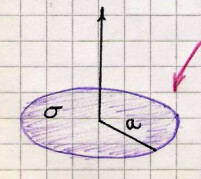
\includegraphics[width=0.25\textwidth]{images/fig_ft1_disco_cargado.jpg}	 


\end{ejemplo}

\begin{ejemplo}{\bf Aros cargados}


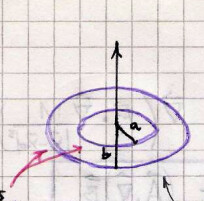
\includegraphics[width=0.25\textwidth]{images/fig_ft1_aros_cargados.jpg}

En este caso la carga total es nula, el monopolo es nulo entonces.
\[
	\lambda_A = \frac{Q}{2 \pi a } \qquad \lambda_B = \frac{Q}{2 \pi b }
\]
de manera que 
\[
	|\lambda_A| = | \lambda_B | \: \frac{b}{a}
\]
El dipolo será nulo respecto del origen y respecto a otros puntos también.
El tensor cuadripolar está caracterizado por un sólo número (luego consideramos a los átomos neutros
monopolar y dipolarmente) $ Q_n = e^{-1} Q_{zz}$.
\notamargen{Algunos momentos cuadripolares nucleares:
Para el $^{14}\mathrm{N}$ es $Q= 7.1\cdot 10^{-2}$ y para el $^{35}\mathrm{Cl}$ es $Q= -7.9\cdot 10^{-2}$}
\end{ejemplo}

\subsection{Momento cuadripolar de un elipsoide}

\[
	\frac{x^2}{A^2} + \frac{y^2}{B^2} + \frac{z^2}{C^2} = 1
\]
y la componente $Q_{11}$ del tensor (que es de traza nula) es
\[
	Q_{xx} = \int \rho( \vbx ) ( 3x^2 - r^2 ) \: d^3x = \rho \int ( 2 x^2 - y^2 - z^2 ) d^3x
\]
donde el tercer término es porque consideramos densidad constante (un elipsoide uniformemente cargado).
Para integrar se hace un cambio de coordenadas
\[
	x'= \frac{x}{A}; \quad y'= \frac{y}{B}; \quad z'= \frac{z}{C};
\]
y entonces se tienen
\[
	Q_{xx} = \frac{q}{5}(2A^2-B^2-C^2) \qquad 
	Q_{yy} = \frac{q}{5}(2B^2-C^2-A^2)  \qquad 
	Q_{zz} = \frac{q}{5}(2C^2-A^2-B^2)
\]
siendo q la carga total. Si el eje $z$ es el de revolución, entonces $A=B$ y se dan
\[
	Q_{xx} = Q_{yy} = \frac{q}{5}(A^2-C^2) \qquad \qquad Q_{zz} = \frac{2q}{5}(C^2-A^2)
\]

\notamargen{Observaciones marginales:
$C_{ij}$ tiene más términos de los que necesito para describir un potencial.
$Q_{ij} = C_{ij}-$ traza, usamos tensor de traza nula.}

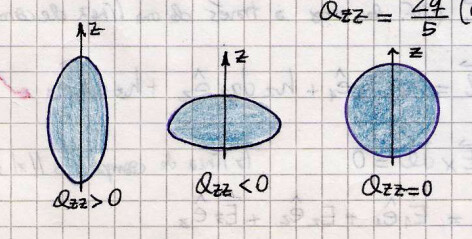
\includegraphics[width=0.4\textwidth]{images/fig_ft1_3elipsoides.jpg}	


\subsection{Interacción de un campo externo con una distribución de carga}

Si tenemos un campo \vb{E} con sus fuentes lejos,


% \begin{figure}[!h]
% 	\begin{center}
	\includegraphics[width=0.4\textwidth]{images/fig_ft1_dipolar3.pdf}	 
% 	\end{center}
% 	\caption{}
% \end{figure}


y que cumple $\divem{E}=0$ y $\rotorm{E}=0$ (irrotacionalidad), se da la siguiente fuerza sobre la distribución
\[
	\vb{F} = \int_V \rho(\vb{x}) \: \vb{E}(\vb{x}) \: dV,
\]
y si \vb{E} no varía demasiado en $V$, entonces podemos representar bien por una serie
\[
	E^\ell(\vb{x}) = E^\ell + x_j \partial_j E^\ell + \frac{1}{2} x_j x_k \partial_j\partial_k E^\ell
\]
entonces 
\[
	F_i = \int_V \rho E_i dV \approx E_i \int_V \rho dV + \int_V \rho  x_j \partial_j E_i dV +
		\frac{1}{2} \int_V \rho x_j x_k \partial_j\partial_k E_i dV 
\]
\notamargen{En la carpeta puse que la integral del cuadrupolo da: $Q_{kj} \partial_k \partial_j E_i$.}
o bien 
\[
	F_i = \int_V \rho E_i dV \approx E_i q + (\vb{p}\cdot\Nabla) E_i  +
		\vb{x}\cdot\left[ (\vb{x}\cdot\Nabla)\Nabla E_i\right]
\]
de lo cual extraemos que el campo interactúa con la carga, el gradiente del campo interactúa con el dipolo
y la divergencia del campo interactúa con el cuadrupolo.
Un campo uniforme entonces no hace fuerza sobre un dipolo.
Para un campo inhomogéneo, el torque $\vb{\Tau} = \vb{x} \times \vb{F}$ se puede escribir como 
\[
	\vb{\Tau} = q\vb{x} \times \vb{E} = \vb{p} \times \vb{E}
\]
donde $\vb{p}\equiv q\vb{x}$ es el momento dipolar y vemos que el torque tiende a centrar el dipolo
según la dirección del campo \vb{E} aunque no lo logra por la agitación térmica.

En la carpeta escribí que reescribía un término de la expansión como
\[
	\frac{1}{2} x_j x_k \partial_j\partial_k E_i =
	\frac{1}{2} \left[ x_j x_k \partial_j\partial_k E_i - \frac{1}{3} r^2 \delta_{ik} \partial_j \partial_k E_i
	\right]
\]
calculo que para lograr que seaa el cuadrupolo la integral. Es la componente sub-$i$ del Laplaciano.


La energía de un dipolo será
\[
	U = -\vb{p}\cdot\vb{E}
\]
entonces
\[
	\vb{F} = -\Nabla U = \Nabla(\vb{p}\cdot\vb{E}) = (\vb{p}\cdot\Nabla)\vb{E} + (\vb{E}\cdot\Nabla)\vb{p}
	+ \vb{p}\times(\rotorm{E}) + \vb{E}\times(\Nabla\times\vb{p})
\]
siendo los últimos tres términos nulos según lo que consideramos previamente de manera que
\[
	\vb{F} = (\vb{p}\cdot\Nabla)\vb{E}.
\]

\subsection{Capa dipolar}

El potencial de un dipolo es
\[
	\phi(\vb{x}) = \frac{ \vb{p}\cdot(\vb{x}-\vb{x}_0) }{|\vb{x} - \vb{x}_0|^3} 
\]
y el potencial de una capa dipolar
\[
	\phi(\vb{x}) = \int_S \frac{ \vb{D}(\vb{x}')\cdot(\vb{x}-\vb{x}') }{|\vb{x} - \vb{x}'|^3} \: dS'
\]
siendo $\vb{D}$ el momento dipolar por área que viene de acuerdo a la definición
\[
	D = \lim_{\substack{\sigma\to\infty \\ \epsilon\to 0}} \: \sigma \: \epsilon
\]
refiérase a la ilustración bajo esta línea. Pero antes algunas cuentas con los dedos
\[
	\delta \phi = \frac{ \delta \vb{p}\cdot(\vb{x}-\vb{x}_0) }{|\vb{x} - \vb{x}_0|^3} 
\]
\[
	\delta \vb{p}(\vbx') = \vb{D}(\vbx') \delta S'
\]
\[
	\int_S d \phi(\vb{x}) = 
	\int_{S'} \frac{ \vb{D}(\vb{x}')\cdot(\vb{x}-\vb{x}') }{|\vb{x} - \vb{x}'|^3} \: dS'
\]

% \begin{figure}[htb]
% 	\begin{center}
	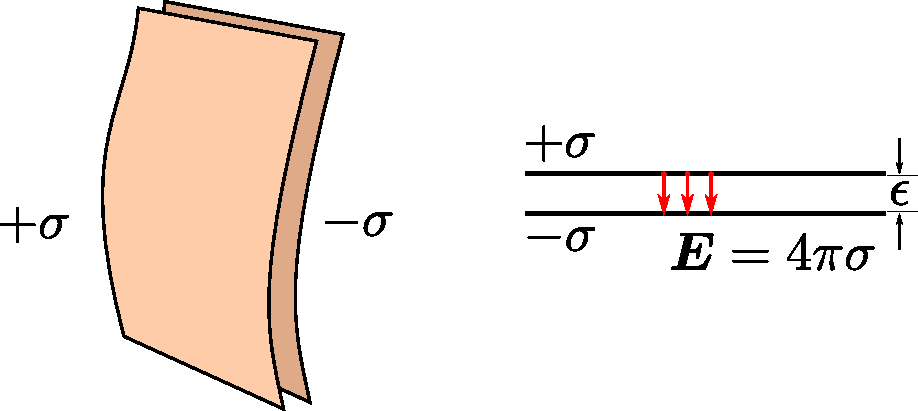
\includegraphics[width=0.75\textwidth]{images/fig_ft1_campo_dipolar3.pdf}	 
% 	\end{center}
% 	\caption{}
% \end{figure}

Veamos algún detalle más sobre la capa dipolar, que está ilustrado en la Figura siguiente.
\[
	\frac{ \vb{D}\cdot(\vb{x}-\vb{x}')}{|\vb{x} - \vb{x}'|^3} dS = 
	\frac{ D \cdot(\vb{x}-\vb{x}')}{|\vb{x} - \vb{x}'|^3} d\vb{S} = 
	- \frac{ D \cos(\theta)}{|\vb{x} - \vb{x}'|^2} dS = 
	- \frac{ D \cos(\theta)}{r^2} dS  
\]

\begin{figure}[htb]
	\begin{center}
	\includegraphics[width=0.6\textwidth]{images/fig_ft1_campo_dipolar1.pdf}	 
	\end{center}
	\caption{}
\end{figure}

\[
	\frac{ \vb{D}\cdot(\vb{x}-\vb{x}')}{|\vb{x} - \vb{x}'|^3} dS = - D d\Omega
\]
puesto que
\[
	\phi(\vb{x}) = -D \int_S d\Omega \qquad \qquad \frac{\cos(\theta)}{r^2}dS \equiv d\Omega
\]

Para las condiciones de contorno se da lo siguiente
\[
	E_2^{\hat{n}} - E_1^{\hat{n}} = 4\pi\sigma
\]
\[
	- \Nabla (\phi_2 - \phi_1)\cdot \hat{n} = 4\pi\sigma
\]
\[
	\dpar{\phi_1 - \phi_2}{\hat{n}} = 4\pi\sigma
\]
\[
	\phi_1 - \phi_2 = 4\pi\sigma\:\epsilon
\]

Y el cálculo del trabajo
\[
	W_{1\to 2} = - q \: 4 \pi \sigma \:\epsilon = q\:( \phi_1 - \phi_2 )
\]
desde donde deducimos que el potencial tiene un salto al surcar la capa dado por 
\[
	\phi_2 - \phi_1 = 4\pi D
\]
Entonces, asociado a una capa dipolar hay un salto de $4\pi D$.

\notamargen{Acá hay que trabajar mejor esto de la capa dipolar en referencia a las BC.
Además saber si lo del $W$ de 1 a 2 es usar la integral de línea por un camino perpendicular
a la surface.}

Para dos chapas infinitas de carga uniforme $\sigma$ pero opuesta el campo eléctrico es nulo 
en todas partes salvo en el interior, donde vale $4\pi\sigma$ (véase ilustración abajo).
Luego el potencial tiene un salto de $4\pi\sigma d$ que se produce a lo largo de la distancia
$d$.

\begin{figure}[htb]
	\begin{center}
	\includegraphics[width=0.4\textwidth]{images/fig_ft1_campo_dipolar2.pdf}	 
	\end{center}
	\caption{}
\end{figure}

Si se considera el límite $\sigma \to \infty$ y $d\to 0$ se tiene una capa dipolar y lo 
que sucede es que la subida apreciable dada por la recta se colapsa a un escalón.


\subsection{Momento dipolar por unidad de volumen}

El potencial de un dipolo es
\[
	\phi(\vb{x}) = \frac{ \vb{p}\cdot(\vb{x}-\vb{x}') }{|\vb{x} - \vb{x}'|^3} 
\]
Suponiendo una distribución continua de dipolos dada por $\vb{P}(\vbx)$, el potencial total debido
a la misma se obtiene de la integración
\[
	\phi(\vb{x}) = \int_V \frac{ \vb{P}(\vb{x}')\cdot(\vb{x}-\vb{x}') }{|\vb{x} - \vb{x}'|^3}  \: dV,
\]
donde $\vb{P}$ es la llamada polarización, el momento dipolar por unidad de volumen, siendo $V$ un volumen
que incluye a la zona de polarización (ver Figura).
\begin{figure}[htb]
	\begin{center}
	\includegraphics[width=0.3\textwidth]{images/fig_ft1_dipolarvol.pdf}	 
	\end{center}
	\caption{}
\end{figure}
Este volumen debe incluir a la misma aunque puede no coincidir con ella.
El potencial se puede escribir como 
\[
	\phi(\vb{x}) = \int_V \vb{P}(\vb{x}')\cdot \Nabla' \left(\frac{1}{|\vb{x} - \vb{x}'|} \right)\: dV
\]
Luego, usando la identidad ID 1 (apéndice) la anterior integral resulta en
\[
	\phi(\vb{x}) = \int_V  \Nabla' \cdot \left( \frac{\vb{P}(\vb{x}')}{|\vb{x} - \vb{x}'|} \right) \: dV
	- \int_V \frac{ \Nabla' \cdot \vb{P}(\vb{x}') }{|\vb{x} - \vb{x}'|} \: dV
\]
y si usamos el teorema de la divergencia en la primera integral se tiene
\[
	\phi(\vb{x}) = \int_S \frac{\vb{P}(\vb{x}')}{ |\vb{x} - \vb{x}'|} \: dS
	- \int_V  \frac{  \Nabla' \cdot \vb{P}(\vb{x}') }{|\vb{x} - \vb{x}'|} \: dV, 
\]
lo que habilita a pensar que el borde del cuerpo polarizado tiene una densidad de carga
de polarización
\[
	\sigma_P = \vb{P}\cdot\hat{n},
\]
y que en el interior existe una carga de polarización volumétrica
\[
	\rho_P = - \Nabla\cdot\vb{P},
\]
siempre y cuando $\divem{P}\neq 0$, es decir que la polarización no sea homogénea.

\begin{ejemplo}{\bf Problema 3}

El problema a resolver se esquematiza en la figura siguiente, donde se ve un dipolo eléctrico
frente a una esfera de radio $a$ conectada a tierra y una carga $q$

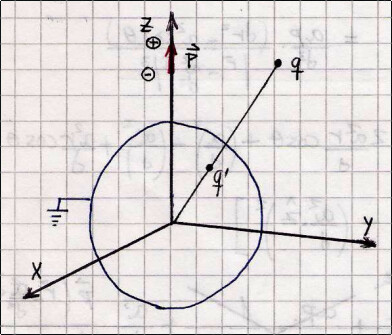
\includegraphics[width=0.3\textwidth]{images/fig_ft1_problema3A.jpg}

El potencial será
\[
	\phi(\vbx) = \int_V \rho(\vbx') G_D(\vbx,\vbx') dV - \frac{1}{4\pi}\int_S \phi \partial_n G_D dS,
\]
pero la última integral será nula puesto que la esfera está puesta a tierra ($\phi=0$ sobre la esfera).
La función de Green para una carga $q$ frente a una esfera será
\[
	 G_D(\vbx,\vbx') = \frac{1}{|\vbx-\vbx'|} - \frac{a}{|\vbx'|}\frac{1}{|\vbx - a^2/r^2 \vbx'|}
\]
donde debe recordarse que en la expresión de la función de Green, 
\[
	G_D(\vbx,\vbx') = \frac{1}{|\vbx-\vbx'|} + F(\vbx,\vbx')
\]
que aporta la geometría del problema, la parte $F$ son las contribuciones debidas a las imágenes.
La densidad de carga será
\[
	\rho(\vbx') = \lim_{\varepsilon\to 0} -q \delta(\vbx' - \vb{d}) + q \delta(\vbx' - \vb{d} - \vb{\varepsilon})
\]
donde el último término debiera expandirse en serie de Taylor (lo cual puede hacerse ahora o después
de integrar). Entonces
\[
	q \delta(\vbx' - \vb{d} ) + q \Nabla \delta(\vbx' - \vb{d}) \cdot \vb{\varepsilon} + ...
\]
y se tiene
\[
	\rho(\vbx') =  \lim_{\varepsilon\to 0} - q \Nabla \delta(\vbx' - \vb{d}) \cdot \vb{\varepsilon} =
	- \vb{p} \cdot \Nabla \delta(\vbx' - \vb{d}).
\]

De esta forma 
\[
	\phi(\vbx) = - \int_V  \vb{p} \cdot \Nabla \delta(\vbx' - \vb{d}) \: G_D(\vbx,\vbx') \: dV =
	-  \vb{p} \cdot \Nabla G_D(\vbx,\vb{d}),
\]
que no es otra cosa que 
\[
	\phi(\vbx) =  \vb{p} \cdot \left. \Nabla_{x'} \left( 
	\frac{1}{|\vbx-\vbx'|} - \frac{a}{|\vbx'|}\frac{1}{|\vbx - a^2/x^2 \vbx'|}
	\right) \right|_{|\vbx'|=|\vb{d}|},
\]
pero se puede intercambiar $x\equiv|\vbx|$ con $x'\equiv |\vbx'|$ así no hay problemas con los diferentes
versores $\hat{x},\hat{x}'$.
Entonces el segundo término de la anterior expresión pasa a ser
\[
	\frac{a}{x} \frac{1}{| x'\hat{x}- a^2/x \:\hat{x}'|} =
	\frac{a}{x} \: \frac{1}{ \left( {x'}^2 + \Frac{a^2}{x}^2 - 2 a^2 \cos( \hat{x}, \hat{x}') \right)},
\]

Teniendo en cuenta este intercambio,
\[
	\phi(\vbx) =  \vb{p} \cdot \left. \Nabla_{x'} \left( 
	\frac{1}{|\vbx'-\vbx|} - \frac{a}{|\vbx|}\frac{1}{|\vbx' - a^2/x^2 \vbx|}
	\right) \right|_{|\vbx'|=|\vb{d}|},
\]
que lleva a 
\[
	\phi(\vbx) = - \frac{\vb{p}\cdot(\vbx-\vbx')}{|\vbx-\vbx'|^3} 
	- \frac{a}{x} \left. \frac{ \vb{p} \cdot ( x^2 \vbx' - a^2 \vb{x} )}{|\vbx' - a^2/x^2 \: \vbx|^3}
	\right|_{|\vbx'|=|\vb{d}|},
\]
donde el primer término es un dipolo y al segundo puede dársele otra forma. En efecto, evaluando
en el punto solicitado se tiene
\[
	\frac{a}{x^3} \frac{ \vb{p} \cdot ( x^2 \vb{d} - a^2 \vb{x} )}{|\vb{d} - a^2/x^2 \: \vbx|^3} = 
	\frac{a}{d^3} \frac{ \vb{p} \cdot ( x^2 \vb{d} - a^2 \vb{x} )}{|\vbx - a^2/d^2 \: \vb{d}|^3}
\]
donde se ha podido intercambiar $d$ con $x$ por la forma de la expresión. Luego, considerando
el ángulo $\theta$ entre \vb{p} y \vb{x} se tiene
\[
	\frac{ap}{d^2} \frac{( x^2 - a^2 /d \: \cos\theta)}{|\vbx - a^2/d^2 \: \vb{d}|^3}
\]
Luego, completando cuadrados en el numerador se puede poner
\[
	\frac{ap}{d^2}\left[\: x^2 - \frac{a^2}{d} x \cos\theta \:\right] =
	\frac{ap}{d^3}\left[\: x^2 - 2 \frac{a^2}{d} x \cos\theta + \frac{a^2}{d} x \cos\theta 
	+ \Frac{a}{d}^2 - \Frac{a}{d}^2 \:\right]
\]
\[
	\frac{ap}{d^2}\left[\: x^2 - \frac{a^2}{d} x \cos\theta \:\right] =
	\frac{ap}{d^2}\left[\: |\vbx - a^2/d \: \hat{z}|^2 + \frac{a^2}{d}\vbx\cdot\hat{z} - 
	\left| \frac{a^2}{d} \hat{z} \right|^2 \:\right]
\]
de manera que finalmente
\[
	\phi(\vbx) =  - \frac{\vb{p}\cdot(\vbx-\vb{d})}{|\vbx-\vb{d}|^3} +
	\frac{ap}{d^2} \frac{1}{|\vbx - a^2/d^2 \: \vb{d}|}+
	\frac{a^3}{d^3} \frac{\vb{p}\cdot(\vbx- a^2/d^2 \: \vb{d})}{|\vbx - a^2/d^2 \: \vb{d}|^3}
\]
y se tienen entonces tres términos que son: un dipolo real, un monopolo imagen y un dipolo imagen.

Notemos entonces que además de haber generado la imagen de un dipolo fue necesaria la imagen de una carga
puntual extra. Si hubiésemos resuelto el problema haciendo la imagen directamente del dipolo hubiera
estado incompleta\footnote{Si se hace la imagen del dipolo considerando sus cargas componentes sale
bien la cosa}.

Por imágenes el problema involucra resolver desde
\[
	\phi(\vbx) = \frac{-q}{|\vbx -\vb{d} |} + \frac{q}{|\vbx -(\vb{d} + \vb{\varepsilon}) |} + 
	\frac{q}{d}\frac{1}{|\vbx - a^2/d^2 \: \vb{d} |} 
	- \frac{q}{(d+\varepsilon)}\frac{1}{|\vbx - a^2/(d+\varepsilon)^2 \: (\vb{d} + \vb{\varepsilon}) |},
\]
y aquí deberían expandirse los denominadores con $\varepsilon\to 0$ mediante Taylor.
En el último término de la expresión anterior convendría permutar $(d+\varepsilon)$ con $x$.
Entonces hay que usar las mismas ideas que en el caso anterior.

Acá hay una observación asociada al figurín bajo estas líneas

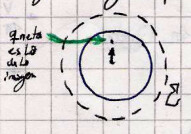
\includegraphics[width=0.3\textwidth]{images/fig_ft1_problema3B.jpg}

Con un problema interior la carga inducida es la carga imagen; porque puedo usar Gauss con una
superficie $\Sigma$ y el campo depende de la carga encerrada real ($\sigma$ inducida).

La parte (c) 
\[
	\dpar{\phi_0}{n} - \dpar{\phi_I}{n} = - 4 \pi \sigma_\text{ind},
\]
y como el segundo término del LHS es cero, se tiene
\[
	\sigma_\text{ind} = - \frac{1}{ 4 \pi } \dpar{\phi_0}{r}(\vbx)
\]
donde la derivada es en esféricas.

La parte (d) es un desarrollo multipolar
\[
	\phi(\vbx) = \frac{Q}{x} + \frac{ \pe{p}{x} }{x^3} + \frac{1}{2} \frac{ \vb{x}^t Q \vbx }{x^5} + ...
\]
Se tienen
\[
	Q = \int_V \rho(\vbx') dV = \frac{ a p }{ d^2 }
\]
que es la carga imagen puntual.
\[
	\vb{p} = \int_V \: \vbx'\rho(\vbx') \: dV = [ -q \vb{d} + q ( \vb{d} + \vb{\varepsilon} ) ] =
	\vb{p} \left( 1  + 2\frac{a^3}{d^3} \right)
\]
que, considerando el primer dipolo, da el aporte de un dipolo más una contribución de la esfera.

\notamargen{Anoté la definición del momento cuadrupolar
\[
	Q_{ij} = \int \: ( 3 x_i x_j - |\vbx|^2 \delta_{ij})\: \rho \: dV
\]}

Puedo tomar ejes principales en $x,y$. Por la simetría de este problema $Q_{xx}, Q_{yy}$ son iguales
de manera que como la traza es nula, con solo calcular $Q_{xx}$ ya tengo todo lo que necesito.

Para el dipolo real (será el momento cuadripolar de un dipolo desplazado del origen)
\[
	Q_{xx} = - q (-d^2 ) + q( -( d + \varepsilon )^2 ) = - 2 p d
\]
donde en el último término se ha hecho el límite $\varepsilon \to 0$.
Para la carga imagen y el diplo imagen serán, respectivamente,
\[
	Q_{xx} = \frac{ap}{d^2} \Frac{a^2}{d}^2 \qquad \qquad 
	Q_{xx} = - 2 \Frac{a^3 p}{d^3} \Frac{a^2}{d}
\]
Sumando todos
\[
	Q_{xx} = - 2 p d \left( 1 + \frac{a^5}{2 d^5} \right),
\]
el último factor es la contribución de la esfera al cuadripolo.

Por superposición, si la esfera estuviera a potencial V como se muestra en el gráfico 

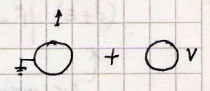
\includegraphics[width=0.3\textwidth]{images/fig_ft1_problema3C.jpg}

se tendría 
\[
	\int_v \rho G_d dV - \frac{1}{4\pi} \int_S \phi \partial_n G_D dS
\]
y la integral de superficie se puede hacer utilizando la ley de Gauss,
\[
	-\frac{V}{4\pi} \int_S E_G dS = \frac{Va}{r}
\]

\notamargen{Anoté por allí que superposición es un Green gráfico.}

Esta última situación no sé bien a qué viene:

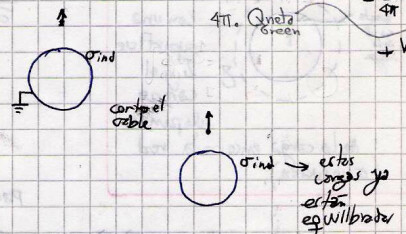
\includegraphics[width=0.3\textwidth]{images/fig_ft1_problema3D.jpg}

Cualquier carga $Q$ que se añada después ya non altera la distribución $\sigma$.

\end{ejemplo}

\begin{ejemplo}{\bf Problema 4}

Aquí lo que sucede es que se generan imágenes en forma recurrente.

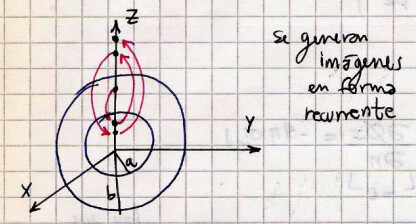
\includegraphics[width=0.3\textwidth]{images/fig_ft1_problema4.jpg}

Podemos agrupar en un cuadro la generación según el orden. Entonces
en cada orden $n$ tendremos un par $(q,r)$ que se construye colocando
la prescripción $(q,r)$ anterior correspondiente al radio ``cruzado''.
Así por ejemplo, el $n=2$ se construye en $r<a$ tomando la prescripción
de $n=1$ con $r<a$ y reemplazando allí el $n=1$ de $r>b$. Consecuentemente,
la prescripción $n=2$ para $r>b$ se construye tomando la $n=1$ de $r>b$ y
reemplazando allí la $n=1$ de $r<a$.

\begin{center}
\begin{tabular}{c|c|c}
$n$ & $r<a$ & $r> b$ \\
\hline
& & \\
1 & $\displaystyle \left( -\frac{aq}{r}, \frac{a^2}{r} \right)$ & 
$\displaystyle \left( -\frac{bq}{r}, \frac{b^2}{r} \right)$ \\
& & \\
2 & $\displaystyle \left( -\frac{a (-qb/r)}{b^2/r}, \frac{a^2}{b^2/r} \right) =
\displaystyle \left( \frac{aq}{b}, \frac{a^2r}{b^2} \right)$ & 
$\displaystyle \left( -\frac{b(-aq/r)}{a^2/r}, \frac{b^2}{a^2/r} \right) = 
\displaystyle \left( \frac{bq}{a}, \frac{b^2r}{a^2} \right) $ \\
& & \\
3 & $\displaystyle \left( -\frac{qa^2}{br}, \frac{a^4}{b^2r} \right)$ & 
$\displaystyle \left( -\frac{qb^2}{ar}, \frac{b^4}{a^2r} \right)$ \\
& & \\
 & ... & ...
\end{tabular}
\end{center}

Siguiendo la recurrencia se tiene 
\[
	n=1,3 : \quad - q \: \frac{a}{r}\Frac{a}{b}^n \quad n \in \mathbb{N}_{+0} \quad r < a
\]
\[
	n=2,4 : \quad q \Frac{a}{b}^n \quad n \in \mathbb{N} \quad r < a
\]
y
\[
	n=1,3 : \quad - q \: \frac{b}{r}\Frac{b}{a}^n \quad n \in \mathbb{N}_{+0} \quad r > b
\]
\[
	n=2,4 : \quad q \Frac{b}{a}^n \quad n \in \mathbb{N} \quad r > b
\]
mientras que para las distancias se obtiene
\[
	n=1,3 : \quad  \: \frac{a^2}{r}\Frac{a}{b}^{2n} \quad n \in \mathbb{N}_{+0} \quad r < a
\]
\[
	n=2,4 : \quad \: r\Frac{a}{b}^{2n} \quad n \in \mathbb{N} \quad r < a
\]
y
\[
	n=1,3 : \quad \: \frac{b^2}{r}\Frac{b}{a}^{2n} \quad n \in \mathbb{N}_{+0} \quad r > b
\]
\[
	n=2,4 : \quad \: r\Frac{b}{a}^{2n} \quad n \in \mathbb{N} \quad r > b
\]

Finalmente todo esto se puede ubicar en una serie para la función de Green, que será
\[
	G_D = \sum_{n=0}^\infty \left[ \frac{\displaystyle - \Frac{a}{x}\Frac{a}{b}^n }
	{ \displaystyle | \vbx - \Frac{a}{x'}^2\Frac{a}{b}^{2n} \vbx'|} + 
	\frac{\displaystyle - \Frac{b}{x}\Frac{b}{a}^n }
	{ \displaystyle | \vbx - \Frac{b}{x'}^2\Frac{b}{a}^{2n} \vbx'|} \right] + 
\]
\[
	\sum_{n=0}^\infty \left[ \frac{\displaystyle \Frac{a}{b}^n }
	{ \displaystyle | \vbx - \Frac{a}{b}^{2n} \vbx'|} + 
	\frac{\displaystyle \Frac{b}{a}^n }
	{ \displaystyle | \vbx - \Frac{b}{a}^{2n} \vbx'|} \right] +
	\frac{1}{|\vbx -\vbx'|}
\]
% Hay que unir estos dos términos.

 
\end{ejemplo}

% =================================================================================================
\section{Desarrollo multipolar para el campo magnético}
% =================================================================================================

Haremos una especie de desarrollo multipolar del potencial vector \vb{A},
\[
	\vb{A}(\vb{x}) = \frac{1}{c} \int_V \frac{\vb{J}(\vb{x}')}{|\vb{x}-\vb{x}'|} \: dV' 
\]
quedándonos a primer orden para $\vbx$ en torno a $\vb{x}'=0$. Es decir, se empleará
\[
	\frac{1}{|\vb{x}-\vb{x}'|} \approx \frac{1}{|\vb{x}|}  + \frac{\vb{x}\cdot\vb{x}'}{|\vb{x}|^3} 
\]
lo cual conduce a
\notamargen{Recordar que Biot \& Savart es para densidad de corriente estacionaria,
i.e. $\divem{J}=0$}
% \[
% 	\vb{A}(\vb{x}) = \frac{1}{c} \int_V \frac{\vb{J}(\vb{x}')}{|\vb{x}|} \: dV' 
% 	+ \frac{1}{c} \frac{ \vb{x} \: }{|\vb{x}|^3} \cdot \int_V \vb{x}' \vb{J}(\vb{x}') \: dV' 
% \]
\[
	\vb{A}(\vb{x}) = \frac{1}{c|\vb{x}|} \int_V \vb{J}(\vb{x}') \: dV' 
	+ \frac{1}{c} \frac{ \vb{x} \: }{|\vb{x}|^3} \cdot \int_V \vb{x}' \vb{J}(\vb{x}') \: dV' 
\]
donde el primer término es nulo lo cual se verá a continuación. En notación indicial la integral
que interesa es 
\[
	\int_V J_i (\vb{x}') \: dV',
\]
luego notemos que 
\[
	\partial_k ( J_k x_i ) = ( \partial_k  J_k ) x_i + J_k \partial_k x_i 
\]
donde el primer término es nulo por ser la divergencia de $\divem{J}$ y el segundo es la delta
de Kronecker de tal forma que
\be
	\partial_k ( J_k x_i ) = J_k \delta_{ki} = J_i. 
	\label{expresion_J}
\ee
El teorema de la divergencia entonces nos asegura que
\[
	\int_V \partial_k ( J_k x_i ) \: dV = \int_S J_k x_i \: dS
\]
donde debe notarse que si la superficie es tal que engloba a todas las corrientes $J$ entonces
ya no hay corriente sobre la superficie y el integrando es nulo.

Se quiere ver que vale 
\[
	\int_V J_i \: x_k \: dV = - \int_V J_k \: x_i \: dV,
\]
y para ello veamos qué le pasa a la divergencia de un tensor de tercer rango, que se puede
escribir
\[
	\partial_l( x_i J_l x_k ) =  \partial_l( x_i J_l ) \: x_k + x_i J_l \:\partial_l( x_k )
\]
usando el resultado anterior \eqref{expresion_J} es
\[
	\partial_l( x_i J_l x_k ) = J_i \: x_k + x_i J_k,
\]
y como es
\[
	\int_V (J_i \: x_k + x_i J_k ) \: dV = 0.
\]
\notamargen{Parece que acá termina la cosa. No me queda nada claro.}
% puede verse porque sale integrando con alguna identidad (?)
% y usando que $\divem{J}=0$. 

Por otra parte, dado que 
\[
	\vbx \times ( \vbx'\times \vb{J}) = (\pe{x}{J})\: \vbx'- \vb{J} \: (\pe{x}{x'} )
\]
se puede aplicar esto en la integración del segundo término
\[
	\int_V x_i J_k x_i' \: dV' = \int_V x_i J_i x_k' \: dV' - \int_V \vbx \times ( \vbx' \times \vb{J} )_k \: dV'
\]
donde el primero aquí será nulo porque es idéntico al anterior, y entonces
\[
	\int_V x_i J_k x_i' \: dV' = - \frac{1}{2} \: \vbx \times \int_V  ( \vbx' \times \vb{J} )_k \: dV',
\]
quedando en deuda la explicación del $1/2$.

\notamargen{Esto habrá que hacerlo bien. La notación está muy poco consistente.}

Este término que resultó nulo correspondería al orden monopolar y su nulidad refleja la no existencia 
de monopolos magnéticos.

Esto conduce a 
\[
	\vb{A}(\vb{x}) = \frac{1}{|\vb{x}|^3} 
	\left[ \left(\frac{1}{2c} \int_V \vb{x}'\times \vb{J} \: dV \right) \times \vb{x} \right] 
\]
y si definimos el corchete como \vb{m} (momento magnético) entonces
\[
	\vb{A}(\vb{x}) = \frac{\vb{m} \times \vb{x} }{|\vb{x}|^3}
\]
en el origen, y 
\[
	\vb{A}(\vb{x}) = \frac{\vb{m} \times (\vb{x}-\vb{x}') }{|\vb{x}-\vb{x}'|^3}
\]
desplazado hacia $\vb{x}'$, las cuales son expresiones a primer orden y que utilizan el gauge de Coulomb, 
$\divem{A}=0$.

De esta manera tendremos
\[
	\mathcal{M}(\vb{x}') = \frac{1}{2c} \left[ \vb{x}' \times \vb{J}(\vb{x}')\right]
\]
que es la magnetización o densidad de momento magnético, y entonces el momento magnético pasa a ser 
\[
	\vb{m} = \int_v \mathcal{M}(\vb{x}') \:dV'.
\]

Ahora se querrá ver qué le pasa al rotor de $\vb{A}$. Para ello se usa la identidad vectorial I2 del apéndice.
Considerando $\vb{m} = \vb{M}$ y $\vb{N} = \vbx / |\vbx|^3 $ se tiene 
\[
	\Nabla \times \left( \frac{\vb{m} \times \vb{x} }{|\vb{x}|^3} \right) =
	\vb{m} \: ( \Nabla \cdot \vbx / |\vbx|^3 ) - \vb{N} \: ( \divem{m} ) +
	( \vbx / |\vbx|^3 \cdot \Nabla ) \: \vb{m} - ( \vb{m} \cdot \Nabla ) \: \vbx / |\vbx|^3,
\]
donde los dos primeros términos son nulos \footnote{El segundo es nulo porque $\vb{m}$ no depende de $\vbx$}. 
Entonces
\[
	\rotorm{A} = -( \vb{m} \cdot \Nabla ) \: \frac{\vbx}{|\vbx|^3} + 4 \pi \delta(\vb{x}) \: \vb{m},
\]
pero el segundo término con la delta no se considerará porque estamos lejos de la distribución de
corrientes\footnote{El término con la delta de Dirac cobra importancia en análisis microscópicos y
cuánticos}. Luego,
\[
	\rotorm{A} = \Nabla \times \left( \frac{\vb{m} \times \vb{x} }{|\vb{x}|^3} \right) =
	-(\vb{m}\cdot\Nabla)\frac{\vb{x}}{|\vb{x}|^3}.
\]
Recordando la expresión para el momento dipolar del campo eléctrico (buscarla) como
\[
	\vb{E}^{(2)} = - ( \vb{p}\cdot\Nabla) \frac{\vbx}{|\vbx|^3},
\]
que llevaba a $\vb{E}^{(2)} = ( 3 (\vb{P}\cdot \hat{n}) \hat{n} - \vb{P} )/ |\vbx|^3$, por analogía
se tendrá
\[
	\vb{B} = \frac{3 (\vb{m}\cdot\hat{n})\hat{n} - \vb{m}}{|\vb{x}|^3},
\]
que nos dice que bien lejos cualquier distribución de corriente localizada \vb{B} se presenta como el 
campo magnético de un dipolo magnético dado por \vb{m}(\vb{x}). Esta aproximación corresponde, por 
supuesto, al primer orden del desarrollo.
El momento magnético puede pensarse entonces como una espirilla.

\subsection{Interpretacion del momento magnético}

Se puede pensar al \vb{m} como una espira plana, lo cual nos provee de una noción intuitiva del 
momento dipolar magnético. 
Entre un punto $\vbx$ del borde y un diferencial de arco $d\Bell$ queda definido un triángulo infinitesimal
cuya área $dA$ será 
\[
	dA = \frac{ 1 }{ 2 } x \: \sin(\alpha) \: d\ell, 
\]
que no es otra cosa que el área de un triángulo (base por altura sobre dos), siendo el área orientada
\[
	\vb{A} = \frac{1}{2} \int_\Gamma \vb{x}\times d\Bell  
\]
y entonces
\[
	\vb{m} = \frac{I}{c}\vb{A}
\]
\begin{figure}[htb]
	\begin{center}
	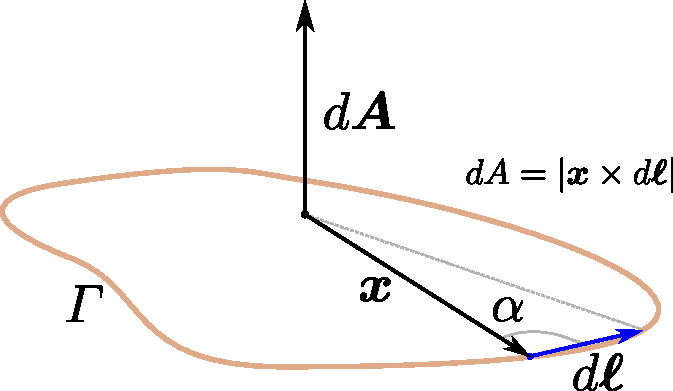
\includegraphics[width=0.5\textwidth]{images/fig_ft1_mmag.pdf}	 
	\end{center}
	\caption{}
\end{figure}

Para convertir un volumen a espira hacemos la transformación del modo usual,
\[
	\vb{m} = \frac{1}{2c} \int_V  \vb{x} \times \vb{J}(\vb{x})  \:dV =
		\frac{I}{2c} \int_\Gamma  \vb{x} \times \:d\Bell
\]
usando que
\[
	\vb{J} \: dV = J \: d\Bell \: dS = \frac{I}{dS} \: d\Bell \: dS = I \: d\Bell 
\]

A modo de ejemplo, para una espira circular de radio $r$ es
\[
	m = \frac{i}{c} \pi r^2.
\]

\subsection{Interacción del campo magnético con una distribución de corriente}

La idea es considerar la fuerza sobre una distribución de corrientes debida a un campo
externo homogéneo.
Hacemos una expansión de Taylor del campo \vb{B} con $|\vb{x}|\ggg|\vb{x}'|$,
\[
	\vb{B} = \vb{B}_0 + (\vb{x}\cdot\Nabla)\vb{B}
\]
y entonces como la fuerza es
\[
	\vb{F} = \frac{1}{c} \int_V \vb{J}(\vb{x}') \times \vb{B}(\vb{x}') \: dV'
\]
\begin{figure}[htb]
	\begin{center}
	\includegraphics[width=0.5\textwidth]{images/fig_ft1_campocorr.pdf}	 
	\end{center}
	\caption{}
\end{figure}
resulta que
\[
	\vb{F} =  \frac{1}{c} \int_V \vb{J} \times \vb{B}_0 \: dV' +
		\frac{1}{c} \int_V \vb{J} \times (\vb{x}'\cdot\Nabla)\vb{B} \: dV'
\]
siendo el primer término nulo.

Mediante identidades vectoriales podemos llegar a una expresión
\[
	\vb{F} = - \Nabla \times \frac{1}{c} \int_V \vb{J}(\vb{x}'\cdot\vb{B}) dV'
\]
y utilizando la demostración previa de que 
\[
	\int \: (\vbx \cdot \vbx') \: \vb{J} \: dV = 
	- \frac{1}{2} \: \vbx \times \int \: \vbx \times \vb{J} \: dV,
\]
resulta que 
\[
	\vb{F} = \Nabla \times \vb{B} \times \frac{1}{2c} \int_V \vb{x} \times \vb{J} \: dV
\]
y entonces, identidades vectoriales mediante,
\[
	\vb{F} = \Nabla\times(\pv{B}{m}) = (\pe{m}{\Nabla})\vb{B} = \Nabla(\pe{m}{B})
\]
Si el campo es homogéneo la fuerza es nula.
Por otra parte, como $\vb{F} = -\Nabla U$ se puede definir energías para los dipolos
de acuerdo con el esquema
\[
	F_m = \Nabla(\pe{m}{B}) \quad \Rightarrow \quad U_m = -\pe{m}{B}
\]
\[
	F_e = \Nabla(\pe{p}{E}) \quad \Rightarrow \quad U_e = -\pe{p}{E}
\]
siendo $U_{m,e}$ la energía de los dipolos en campos externos.

La fuerza de un campo $\vb{B}$ externo sobre una distribución de corrientes es el gradiente de cierta
energía
\[
	\vb{F} = \Nabla(\vb{m}\cdot\vb{B}) = (\vb{m}\cdot\Nabla)\vb{B}
\]
de donde se ve claramente que si \vb{B} es uniforme entonces la fuerza es nula.
\vb{m} es una constante que depende de la distribución de corrientes.

\begin{ejemplo}{\bf Problema 6b}

Ahora $ a \ll L $ y por la simetría de rotación son convenientes coordenadas cilíndricas.
La simetría reclama que no hay dependencia en $ \vp $ ni componente $B_\vp$ de manera que
\[
	\vb{B}(r,z) = B_z(r,z) \zver + B_r(r,z) \rver
\]
Considerando una expansión de Taylor para $r$ pequeños
\[
	B_z(r,z) \approx B_z(0,z) + \left.\dpar{B_z}{r}\right|_{r=0} r\qquad \qquad 
	B_r(r,z) \approx B_r(0,z) + \left.\dpar{B_r}{r}\right|_{r=0} r
\]

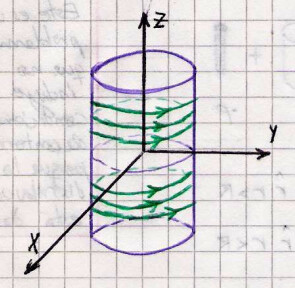
\includegraphics[width=0.4\textwidth]{images/fig_ft1_problema_6b.jpg}

La simetría dice también que  $B_r(0,z) = 0$ y utilizando la divergencia nula $\divem{B}=0$ del campo en
cilíndricas se tiene 
\[
	\frac{1}{r} \dpar{rB_r}{r} + \dpar{B_z}{z} = 0,
\]
o bien
\[
	\dpar{B_r}{r} = - \dpar{B_z}{r} - \left.\dpar{B_z}{r}\right|_{r=0}
\]
y evaluando en $r=0$ se obtiene [CHECK ESTO]
\[
	\left. \dpar{B_r}{r} \right|_{r=0} = 
	- \frac{1}{2} \left. \dpar{B_z}{r} \right|_{r=0}
\]
Se obtiene una expresión algo más general que la que se hubo obtenido (la de la clase pasada, que es la
del capítulo 1)  que utilizaba $ L \to \infty $.
 
\end{ejemplo}

\begin{ejemplo}{\bf Problema 11}

Este es un problema que no incluye condiciones de contorno porque la distribución de carga está dada.
Es un cilindro infinito.
Si hacemos el potencial $\vp$ aquí vemos que revienta lo cual se debe a que la distribución de carga
es infinita.

El arreglo es el de la figura

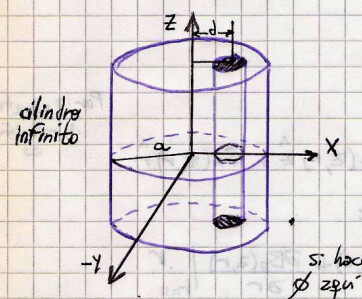
\includegraphics[width=0.375\textwidth]{images/fig_ft1_problema_11a.jpg}

También se puede pensar de la siguiente forma

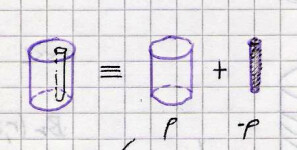
\includegraphics[width=0.5\textwidth]{images/fig_ft1_problema_11b.jpg}

El campo para un cilindro de radio $R$ centrado en $r=0$ es 
\[
	\vb{E}  = 
	\begin{cases} 
		\displaystyle \frac{2 \pi a^2 \rho }{r} \rver & \qquad r \geq R  \\
		\\
		2 \pi r \rho \rver & \qquad r < R
	\end{cases}
\]
Escribiendo el campo interno como 
\[
	2 \pi r \rho \rver = 2 \pi \rho \: \vb{x},
\]
donde $\vbx = r \rver $ es el vector que vive en el plano horizontal, se puede trasladar el cilindro
así 
\[
	2 \pi \rho ( \vb{x} + d \xver )
\]
y entonces el campo dentro del cilindro es
\[
	\vb{E} = 2 \pi \rho d \xver.
\]

\notamargen{Hay que mirar la práctica porque esto está confuso.}

Para la parte (b) se considera

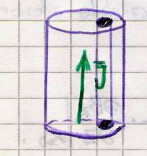
\includegraphics[width=0.2\textwidth]{images/fig_ft1_problema_11c.jpg}

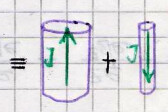
\includegraphics[width=0.3\textwidth]{images/fig_ft1_problema_11d.jpg}

\[
	B(r) 2 \pi r = \frac{4\pi}{c} \pi r^2 j,
\]
pero $\vb{B}$ es en $\phiver$ y entonces
\[
	\vb{B} = \frac{2\pi r j}{c} \frac{\phiver}{r} = \frac{2\pi j}{c} ( -y \xver + x \yver )
\]
de manera que el campo total, que es la suma de los campos del cilindro grande
y del pequeño, será
\[
	\vb{B} = \frac{2\pi j}{c}( -y \xver + d\yver + x \yver ) - \frac{2\pi j}{c}( -y \xver + x \yver ),
\]
o bien
\[
	\vb{B} = \frac{2\pi j}{c} d \yver.
\]
 
\end{ejemplo}

\begin{ejemplo}{\bf Problema 13}

Esfera central a tierra, esfera externa con densidad superficial $\sigma$.
La siguiente equivalencia es posible

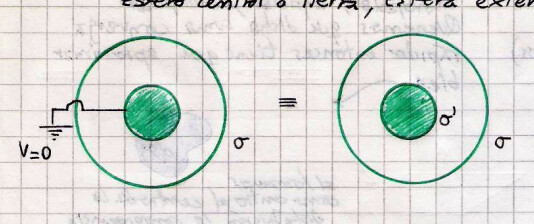
\includegraphics[width=0.5\textwidth]{images/fig_ft1_problema_13a.jpg}

Luego, esto se resuelve así, usando la simetría esférica y la ley de Gauss $ \int \vb{E}\cdot d\vb{S} = 4 \pi Q$
se tienen
\[
	4 \pi r^2 E = \begin{cases} 
	               0 \\
	               4 \pi a^2 \sigma
	              \end{cases}
	\qquad 
	4 \pi r^2 E = \begin{cases} 
	               0 \\
	               4 \pi b^2 \sigma'
	              \end{cases} 
\]
\[
	\vb{E} = \begin{cases}
	          \displaystyle 4 \pi \frac{\sigma a^2 + \sigma' b^2 }{r^2} \rver \quad & r > b \\ 
	          \\
	          \displaystyle 4 \pi \frac{\sigma' b^2}{r^2} \rver \quad & a < r < b \\
	          \\
	          0 & r < a 
	         \end{cases}
\]
El potencial será
\[
	V = \begin{cases}
	          \displaystyle 4 \pi \frac{\sigma a^2 + \sigma' b^2 }{r} + C_1 \quad & r > b \\ 
	          \\
	          \displaystyle 4 \pi \frac{\sigma' b^2}{r}  + C_2 \quad & a < r < b \\
	          \\
	          C_3 & r < a 
	         \end{cases}
\]
y al pedir continuidad para el mismo, se tienen 
\[
	C_1 = 0, \qquad C_2 = 4 \pi \sigma, \qquad C_3 = 0 
\]
donde en la última está metida la $\sigma'$ que hace nulo el potencial $V$ sobre la esfera
interna. Así, finalmente
\[
	V = \begin{cases}
	          \displaystyle 4 \pi \frac{\sigma a (a-b)}{r} \quad & r > b \\ 
	          \\
	          \displaystyle 4 \pi \frac{\sigma a (r-b)}{r} \quad & a < r < b \\
	          \\
	          0 & r < a 
	         \end{cases}
\]

Una serie de diagramitas a descular siguen:

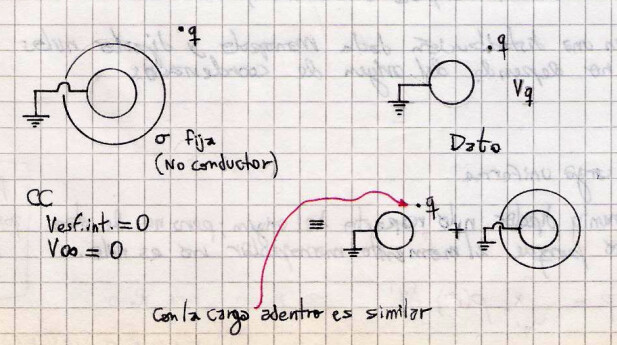
\includegraphics[width=0.5\textwidth]{images/fig_ft1_problema_13b.jpg}
 
\end{ejemplo}



% =================================================================================================
\section{Perturbación por un conductor sobre un campo eléctrico uniforme}
% =================================================================================================

Se tiene un campo uniforme con $Q,R \to \infty$ pero con $2Q/R^2 = cte$, según se ve en la Figura.


El potencial $\phi$ de la esfera es constante por ser conductor.
Puedo definir 
\[
	\phi|_{esf} \equiv 0
\]
pues $\phi(\infty)\neq 0 $ porque hay densidad de carga $\rho$ en el infinito.

\begin{figure}[htb]
	\begin{center}
	\includegraphics[width=0.4\textwidth]{images/fig_ft1_perturbacion1.pdf}	 
	\end{center}
	\caption{}
\end{figure}
Para la carga superior,
\[
	\phi_1 = \frac{-Q}{|\vb{x} - R\hat{z}|} + \frac{a/R Q}{|\vb{x} - a^2/R\hat{z}|}
\]
mientras que para la inferior
\[
	\phi_2 = \frac{Q}{|\vb{x} + R\hat{z}|} + \frac{ a/R Q}{|\vb{x} + a^2/R\hat{z}|}
\]

Recordemos que
\[
	(1+\alpha)^{(-1/2)} \approx 1 - \frac{1}{2}\alpha \qquad \alpha \ll 1
\]
y podemos trabajar el denominador
\[
	|\vb{x} - R\hat{z}| = \sqrt{ x^2 + R^2 - 2Rx\cos(\theta)}
\]
\[
	\frac{1}{|\vb{x} - R\hat{z}|} = \frac{1}{\sqrt{ x^2 + R^2 - 2Rx\cos(\theta)}} =
	\frac{1}{R(1 + x^2/R^2 - 2x/R\cos(\theta))^(1/2)}
\]
\[
	\frac{1}{|\vb{x} - R\hat{z}|} \approx \frac{1}{R}\left(1+ \frac{x}{R} \cos(\theta) \right)
\]
de manera que luego
\begin{multline*}
	\phi(r) \approx Q\left[ \frac{1}{R}\left(1+ \frac{x}{R} \cos(\theta) \right) + 
	\frac{a}{Rx}\left(1+ \frac{a^2}{Rx} \cos(\theta) \right) + \right. \\
	\left. \frac{1}{R}\left(1 - \frac{x}{R} \cos(\theta) \right) -
	\frac{a}{Rx}\left(1 - \frac{a^2}{Rx} \cos(\theta) \right) \right]
\end{multline*}
\[
	\phi(x) \approx -\frac{2Qx}{R^2} \cos(\theta) + \frac{2a^3Q}{R^2x^2}\cos(\theta)
\]
y haciendo $x\equiv r$ y tomando el límite,
\[
	\phi(r) = -E_0 r \cos(\theta) + E_0\frac{a^3}{r^2} \cos(\theta)
\]
y la carga total sobre la esfera es nula puesto que estuvo aislada todo el tiempo.
Respecto de la Figura, si hacemos un Gauss en la zona indicada se obtiene $Q_n=0$,
entonces $\phi(r=a)=0$.

\begin{figure}[htb]
	\begin{center}
	\includegraphics[width=0.2\textwidth]{images/fig_ft1_perturbacion3.pdf}	 
	\end{center}
	\caption{}
\end{figure}

El segundo término es como un dipolo puntual,
\[
	E_0\frac{a^3}{r^2} \cos(\theta) = E_0\frac{a^3 \hat{z}\cdot\vb{r}}{r^3} 
\]
donde
\[
	\vb{p} \equiv E_0 a^3 \hat{z}
\]



\begin{notasfinales}

\label{notas_carga_frente_a_esfera}
\item{ \bf Sobre el problema de la carga frente a la esfera conductora a tierra}

Decíamos que esta solución se puede obtener de manera más heurística, como lo hace Jackson? [CITA],
a partir de la expresión en 
\[
	\frac{q}{\sqrt{ a^2 + y^2 - 2 \: a \: y \:\cos{\gamma}} } +
	\frac{q'}{\sqrt{ a^2 + y'^2 - 2 \: a \: y' \: \cos{\gamma} }} = 0,
\]
se podría intentar forzar que el segundo denominador sea idéntico al primero para lo cual se puede multiplicar
arriba y abajo por el factor $(y/a) $
\[
	\frac{q}{\sqrt{ a^2 + y^2 - 2 \: a \: y \:\cos{\gamma}} } +
	\frac{q' (y/a) }{ y/a \sqrt{ a^2 + y'^2 - 2 \: a \: y' \: \cos{\gamma} }} = 0
\]
lo que conduce a
\[
	\frac{q}{\sqrt{ a^2 + y^2 - 2 \: a \: y \:\cos{\gamma}} } +
	\frac{q' (y/a) }{\sqrt{ y^2 + y^2y'^2/a^2 - 2 \: y^2/a \: y' \: \cos{\gamma} }} = 0
\]
y esta ecuación se satisface si $ y y'= a^2 $ y si $ q = - q' (y/a)$, que es justamente la solución
encontrada previamente de un modo más tradicional.

También es interesante considerar algunos casos límite y ver que se recuperan resultados y comportamientos
familiares. Si $ q $ está localizada muy cerca de la superficie de la esfera, i.e. $ |\vb{y}| \approx a + \varepsilon $
resultan $ y' \approx a - \varepsilon $ y $ q' \approx -q + ( \varepsilon / a ) q $ que son exactamente los
resultados para una carga frente a un plano conductor (si despreciamos la cantidad infinitesimal $( \varepsilon / a )$).
Muy cerca de la superficie de la esfera la carga {\it ve} un plano infinito.


\end{notasfinales}


% \bibliographystyle{CBFT-apa-good}	% (uses file "apa-good.bst")
% \bibliography{CBFT.Referencias} % La base de datos bibliográfica

\end{document}
